\documentclass[10pt,a4paper,final]{report}
\usepackage[utf8]{inputenc}
\usepackage[english]{babel}
\usepackage{amsmath}
\usepackage{amsfonts}
\usepackage{amssymb}
\usepackage{tikz}
\usepackage{multirow}
\usepackage{gensymb}
\usepackage{graphicx}
\usepackage{caption}
\usepackage{subcaption}
\usepackage{wrapfig,floatrow}
\usepackage{listings}   
\usepackage[numbered,framed,final]{mcode}
\graphicspath{ {images/} }
\author{Alessio Russo}
\title{Dynamics of Mechanical Systems - Project}
\begin{document}
\maketitle
\tableofcontents
\newpage
\section{Introduction}
\subsection{Project Description}
The aim of this report is to outline the modelling and the analysis of a single span metallic truss bridge.
\\
The figures below show a metallic bridge and its plane model.
\\
\begin{figure}[h]
\centering
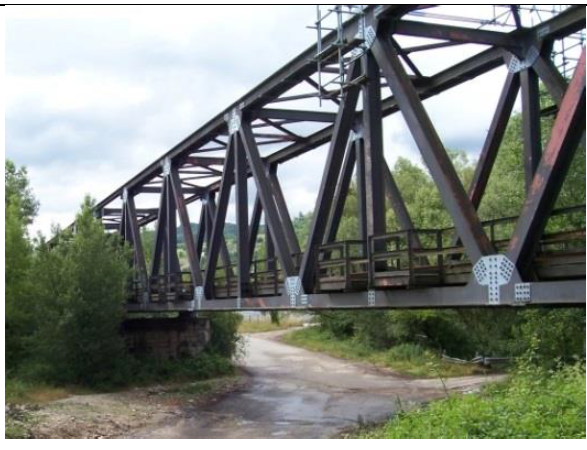
\includegraphics[scale=0.8]{bridge_sample1}
\label{fig:bridge1}
\caption{Example of a truss bridge}
\end{figure}
\begin{figure}[!]
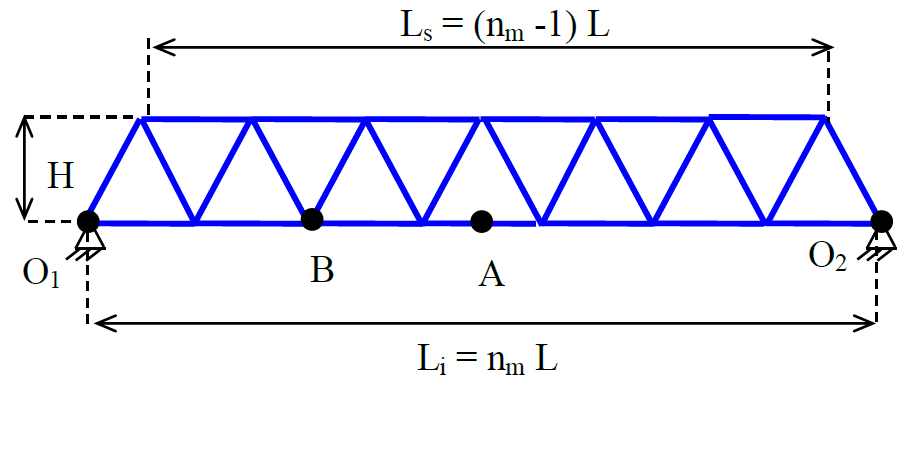
\includegraphics[width=1\textwidth]{bridge_model1}
\caption{Plane model of a truss bridge}
\label{fig:bridge2}
\centering
\end{figure}
\newpage
\subsection{Project Scope}
Various requests need to be fulfilled in order to complete the project. Here they are briefly described:
\begin{enumerate}
\item A FEM model for the bridge needs to be developed. The model has to be valid in the frequency range $f \in [0,15]$ Hz.
\item Compute the system’s natural frequencies and related modes of vibration in the frequency range $f \in [0,15]$ Hz.
\item { Compute the following frequency response functions (FRF) in the frequency range $f \in [0,15]$ Hz with step $\Delta f = 0.01$ Hz:
\begin{enumerate}
\item Vertical displacement of point $A$ produced by a vertical force on point $A$.
\item Vertical displacement of point $B$ produced by a vertical force on point $A$.
\item Vertical acceleration of point $A$ produced by a vertical force on point $B$.
\item Vertical acceleration of point $B$ produced by a vertical force on point $B$.
\end{enumerate}
}
\item {Compute the bridge response due to a seismic motion of the ground:
\begin{enumerate}
\item The spectrum of the input displacements $yO1$, $yO2$.
\item The spectrum of the vertical displacements of points $A$ and $B$.
\item The time histories of the vertical displacements of points $A$ and $B$.
\item The spectrum and the time histories of the vertical accelerations of points $A$ and $B$.
\end{enumerate}
}
\item {Considering the passage with constant speed $V$ of a sequence of moving concentrated loads with distance of $26 m$ from one another, discuss the possibility of producing a resonance condition in the bridge for the specified values of the train's speed $V$. To this end, consider an infinite sequence of moving load (approximation of a long train).}
\item {Either the 6.a or 6.b can be done:
\begin{enumerate}
\item {Define a structural change that allows for a 20\% increase of the first natural frequency of the bridge. To this aim, the total bridge mass must not increase more than 3\%. It’s not allowed to change the span length, to change the material, to add constraints. In case of variation of the beams cross-section, all of the inertial and elastic parameters (m, EA, EJ) must change according to the new cross-section dimension and shape, which has to be chosen among the standard metallic section provided in the tables of standardised geometric properties for beam sections made available on BeeP.}
\item { Define a structural change of the bridge constrains that allows for a 15\% reduction of the maximum amplitude of vibration evaluated at point A when the bridge is subjected to the seismic excitation described at point 4).}
\end{enumerate}
}
\end{enumerate}
\newpage
\subsection{Project Data}
The bridge, as shown in figure \ref{fig:bridge2}, has two constraints:
\begin{enumerate}
\item Hinge in $O_1$.
\item Cart in $O_2$.
\end{enumerate}
Moreover, it is necessary to analyse the vertical displacement of  nodes A, B. \\ \\
The data provided to describe the bridge is briefly summarised in the following table:
\\ \\
\begin{tabular}{ |l|l|l| }
\hline
\multicolumn{3}{ |c| }{\textbf{Geometric Data}} \\ \hline
Length of base for one module $L$ & $[m]$ & $10$ \\ \hline
Modules number $n_m$ &  & $7$ \\ \hline
Bottom chord total length $L_i$ & $[m]$ & $70$ \\ \hline
top chord total length $L_s$ & $[m]$ & $60$ \\ \hline
Bridge height $H$ & $[m]$ & $2.8$ \\ \hline

\multicolumn{3}{ |c| }{\textbf{Properties bottom chord}} \\ \hline
Cross section type &  & IPE400 \\ \hline
$A$ &$[cm^2]$ & $84.46$ \\ \hline
$J$  & $[cm^4]$ & $23130$ \\ \hline

\multicolumn{3}{ |c| }{\textbf{Properties top chord}} \\ \hline
Cross section type &  & IPE400 \\ \hline
$A$ & $[cm^2]$ & $84.46$ \\ \hline
$J$  & $[cm^4]$ & $23130$ \\ \hline

\multicolumn{3}{ |c| }{\textbf{Properties diagonal beams}} \\ \hline
Cross section type &  & HEA160 \\ \hline
$A$ &$[cm^2]$ & $38.77$ \\ \hline
$J$  & $[cm^4]$ & $1673$ \\ \hline

\multicolumn{3}{ |c| }{\textbf{Material: Steel - Coefficients}} \\ \hline
$\rho$ & $[\frac{kg}{m^3}]$ & $7800$ \\ \hline
$E$ & $[\frac{N}{m^2}]$ & $2.06\cdot 10^{11}$ \\ \hline
$\alpha$  & $[s]$ & $0.2$ \\ \hline
$\beta$  & $[s^{-1}]$ & $10^{-4}$ \\ \hline
\end{tabular}
\\ \\ \\
Furthermore, it is assumed that the structural damping is proportional, under the proportional damping assumption.\\ Hence $\exists \alpha, \beta \in \mathbb{R} : [R] =\alpha[M]+\beta[K]$, where $[R]$ is the damping matrix, $[M]$ is the mass matrix and $[K]$ is the stiffness matrix.
\\ \\
Notice that the length of the diagonal beams $L_d$ is not given. We can deduce some relationships:
$$H = L_{d}sin(\theta) \quad 5 = L_{d}cos(\theta)$$
Follows that: 
\begin{align*}
\theta = tan^{-1}\Big(\frac{H}{5}\Big) \approx 29.25 \degree 
\quad L_{d} = \frac{5}{cos(\theta)} \approx 5.73 m
\end{align*}
Parameters also have to be converted to the appropriate dimensional units.
\newpage
\section{Project}
\subsection{FEM Model}
In order to develop a convincing FEM model we have to thoroughly understand under which conditions a nodal section has to be inserted into the model. It is known that a nodal section must be inserted in the following situations:
\begin{enumerate}
\item Whenever there is a variation in the beam properties.
\item Intersection of 2 or more beams, with different axis direction.
\item Presence of a concentrated element (spring, mass, damper, force).
\item Whenever the displacement of a certain point has to be known.
\end{enumerate}
Other rules may be applied, but one of the most important is the following:
\begin{itemize}
\item {In case of  statics loads the approximation of the system motion is the exact solution. Whilst for dynamic loads, in order to get an acceptable approximation of the actual displacement of the systems, each finite element has to work in the range of frequencies well below their first resonance (Quasi static range).
}
\end{itemize}
To ensure a good approximation of the solution, then the following has to be satisfied: $\omega_{k} \gg \Omega_{max}$, where $\omega_{k}$ is the first resonance of the finite element.
\\
$\omega_{k}$ can be calculated from the following formula,  which corresponds to the pinned-pinned case of a beam:
$$\omega_{k} =  \Big(\frac{\pi}{L_{k}}\Big)^2 \sqrt{\frac{EJ_k}{m}}$$
In our particular problem $\Omega_{max} = 2\pi \cdot15$, it follows that:
$$\Big(\frac{\pi}{L_{k}}\Big)^2 \sqrt{\frac{EJ_k}{m}} >> 2\pi \cdot15$$
Hence:
$$L_k \ll \sqrt{\frac{\pi}{2 \cdot 15} \sqrt{\frac{EJ_k}{m}}} = L_{max}$$
How \textit{small} should be $L_k$ when compared to $L_{max}$? There are few rules, described in the appendix. Those rules are:
\begin{itemize}
\item \textit{Half-Power}: $L_k$ is approximated up to the frequency where the first resonance in $\omega_k$ should have half the power.
\item \textit{Derivative rule}: $L_k$ is approximated up to the frequency where the slope of the FRF magnitude is approximately the value given by the user (e.g. $-0.5$).
\item \textit{Frequency Range}: $L_k$ is approximated up to $k\Omega_{max}$, where $k$ is a value given by the user.
\end{itemize}
Using the last rule, with $k=5$, follows that $\omega_{k} =5 \Omega_{max}$. Since the properties of the beams change if we consider diagonal beams, it follows that we have $L_{k,i}, i=1,2$. \\ Specifically $L_{k,1} \approx 4.22 m$, $L_{k,2} \approx 2.66 m$, which are rounded down to \\ $L_{k,1} = \frac{10}{3}, L_{k,2}=2$. In this way we also have nodal sections in A and B.
\\ \\
Once the length is found it is possible to set up the model by writing all of the parameters associated with the nodes and the beams on a file. This however may require a very long time if high precision is needed. For this reason I developed a matlab software, which given the position of the beams on a (x,y) reference system, their rotation with respect to the (x) axis, and lastly their parameters, is capable of automatically producing a FEM model when the frequency range and the accuracy are provided, which we discussed beforehand.


\begin{wrapfigure}{r}{0.4\textwidth}
  \begin{center}
    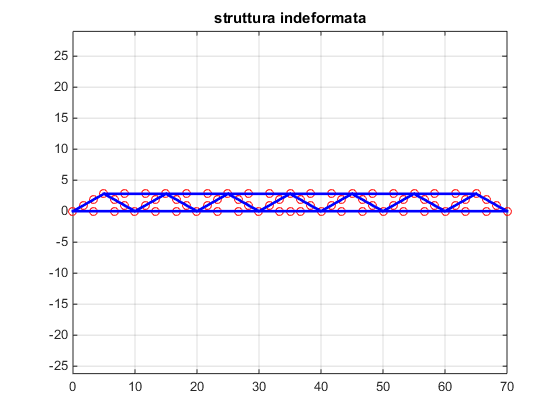
\includegraphics[scale=0.4]{undeformed_structure}
  \end{center}
  \label{fig:femmodel}
  \caption{Fem Model}
\end{wrapfigure}

Moreover, this tool makes it possible to add nodes wherever we want in the beams.
The development of this tool has undergone several steps:
\begin{enumerate}
\item Define what is the geometric model of a system and define what is a node.
\item For each beam calculate, accordingly to the parameters, how many nodes it needs to work in the range of frequencies provided by the user.
\item Join all the beams: remove all duplicated nodes (this may require to reduce precision of the geometric position of a node).
\item Add all the nodes that the user whishes to include, apply the constraints.
\item Write on file the FEM model.
\end{enumerate}

\begin{wrapfigure}{l}{0.5\textwidth}
  \begin{center}
    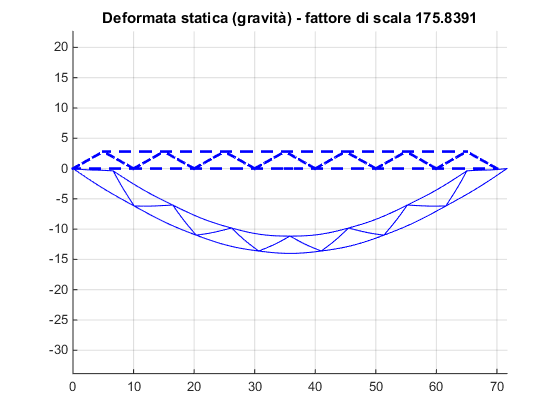
\includegraphics[scale=0.4]{gravity_deformation}
  \end{center}
  \label{fig:gravitydeformation}
  \caption{Static analysis: structure gravity deformation}
\end{wrapfigure}

In this way it was possible to developed a FEM Model where the first frequency of the system lies over $100Hz$. The software produced a FEM Model with $70$ nodes and $82$ beams, as shown in figure \ref{fig:femmodel} (the coefficient used in the tool was 7, to not have too many nodes). \\ \\
Moreover, it is possible to check the static deformation due to gravity in order to make a first check of the validity of the model. The gravity deformation can be seen in figure \ref{fig:gravitydeformation}, which is scaled of a factor $175.8$. Looking at the vertical displacement, we see that node $A$ (which is node $32$ in our model), is the one which presents maximum displacement being in the middle of the bridge, with a value of $y \approx -7.968\cdot 10^{-2} m = -7.968 cm$.
\\ \\
$O_1$ is a hinge and as such it's constrained in the $x,y$ coordinates. In fact said hinge has $0$ displacement for this position. 
Same check goes for $O_2$, which is a kart, and is therefore only constrained in the $y$ direction having $0$ displacement in that direction as expected. \\ \\
From the FEM Model we can retrieve the $[M],[R],[K]$ matrices, which are of dimension $N \times N$, where $N=\text{\# of nodes} \times \text{indipendent coordinates}$, which is $N=70\times 3 = 210$ xindependent coordinates. From those we have to remove the constrained displacements, which are $3$. Therefore the degrees of freedom are $n=3N-p = 210-3=207$.
\\ \\
The matrices are symmetric, and can be splitted into 4 submatrices, like $[M]_{ff}, [M]_{fc}, [M]_{cf}, [M]_{cc}$, thanks to the division of the nodes from the constrained ones to those which are not constrainted $\underline{x}= (\underline{x}_{f}, \underline{x}_{c})^T$. \\ \\
Finally, also the matrix \textbf{IDB} can be retrieved from the software, which is the matrix that indexes the displacements ($x,y,\theta$) of the nodes: $\textbf{IDB}(32,2)$ is the $y$ displacement of node $32$.
\\ \\
The total mass is $10990.4209 Kg$.
\newpage
\subsection{System's natural frequencies and mode of vibrations}
To compute the natural frequencies of a system we can make the $dmb_fem$ software or make a code to automatically calculate it. It's straightforward to implement:
\begin{lstlisting}
[v,d]=eig(Mff\Kff);
[omega,I]=sort(sqrt(diag(d)));
freq=omega/2/pi;
\end{lstlisting}
It's worth to notice that the damping was not taken into account while calculating the natural frequencies, due to the fact that it doesn't affect the natural frequencies to enough an extent. Even so it can be considered by setting $\underline{z}=\underline{\dot{x}}$:
\begin{lstlisting}
Anew = [zeros(nf,nf), eye(nf,nf); -Mff\Kff, -Mff\Rff];
shapes2,puls2]=eig(Anew);
[omega,I]=sort( diag(puls2) );
freq = unique(abs(imag(omega)/(2*pi)));
\end{lstlisting}
By using the tool the first natural frequencies in the range $[0,15]Hz$ are:
\begin{enumerate}
\item Frequency $1.9701 Hz$, with relative mode of vibration displayed in figure \ref{fig:mode1}.
\item Frequency $6.8843 Hz$ and mode of vibration displayed in figure \ref{fig:mode2}.
\item Frequency $12.2399 Hz$ and mode of vibration displayed in figure \ref{fig:mode3}.
\item Frequency $14.3477 Hz$ and mode of vibration displayed in figure \ref{fig:mode4}.
\item Frequency $14.3538 Hz$ and mode of vibration displayed in figure \ref{fig:mode5}.
\end{enumerate}
Since the modes of vibration have a sinusoidal shape, it's obvious that for lower frequencies the amplitude assumes the meaning of being a 'mean' value. Moreover, it's important to understand the effect of the constrained nodes on the natural frequencies.\\ \\
Having a kart on $O_2$ implies that the vibrations can extend on the x axis over the bridge length, thus reducing the amplitude of the oscillations. \\ \\
Furthermore, adding more constraints to $O_2$ implies only that the bridge oscillates at higher frequencies, since  constant modes (lower frequencies) are constrained. \\ \\

In the various figures we can also see the nodal points, which are points that have a 0 mode vibration when a force is applied on them, that mode of vibration is $0$ for that point.
\newpage
\begin{figure}[h]
        \centering
        \begin{subfigure}[t]{0.3\textwidth}
                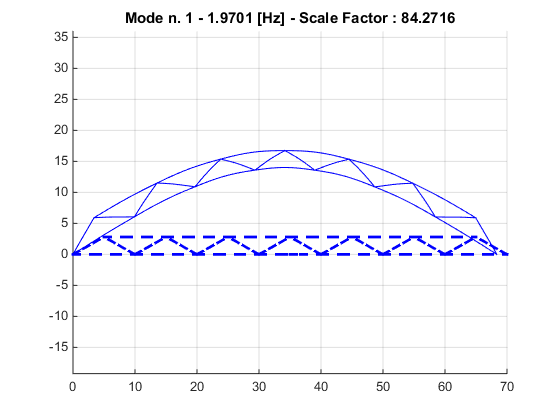
\includegraphics[width=\textwidth]{mode1}
                \caption{$1$-st mode}
                \label{fig:mode1}
        \end{subfigure}%
        \begin{subfigure}[t]{0.3\textwidth}
                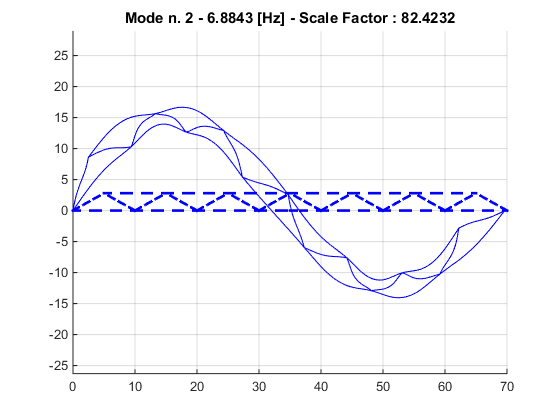
\includegraphics[width=\textwidth]{mode2}
                \caption{$2$-nd mode}
                \label{fig:mode2}
        \end{subfigure}
        \begin{subfigure}[t]{0.3\textwidth}
                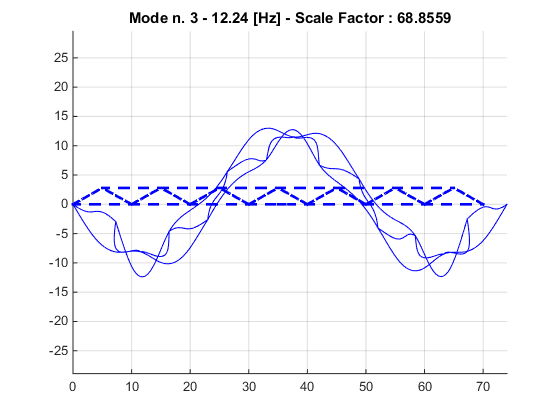
\includegraphics[width=\textwidth]{mode3}
                \caption{$3$-rd mode}
                \label{fig:mode3}
        \end{subfigure}
        \\
        \centering
        \begin{subfigure}[b]{0.3\textwidth}
                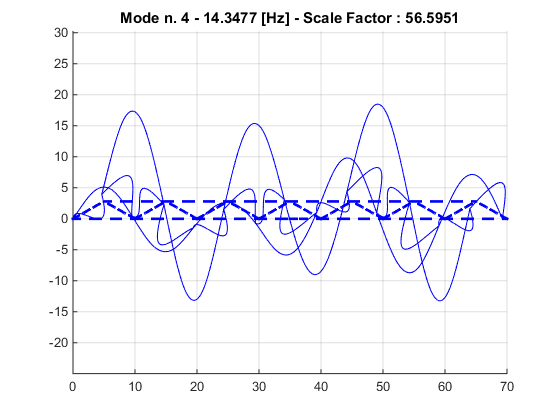
\includegraphics[width=\textwidth]{mode4}
                \caption{$4$-th mode}
                \label{fig:mode4}
        \end{subfigure}%
        \begin{subfigure}[b]{0.3\textwidth}
                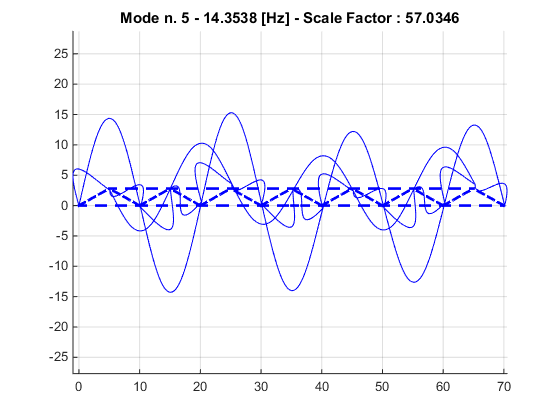
\includegraphics[width=\textwidth]{mode5}
                \caption{$5$-th mode}
                \label{fig:mode5}
        \end{subfigure}
        \caption{Modes of vibration for $f \in [0,15]Hz$} \label{fig:modes}
\end{figure}
\newpage
\subsection{Frequency responce functions}
In this section we have to analyse the FRFs of the point $A,B$ for the displacement and the acceleration. \\ To do so we have to calculate for each frequency the amplitude and the phase of the response, in order to obtain the bode plot of the transfer function, which is equal to sending an impulse of amplitude $1$ as input. \\
A sample matlab code to do so is:
\begin{lstlisting}
df = 0.01;
frequencies = (0:df:15)';
F= zeros(nf,1); F(NA,1) = 1; %NA is the idb(32,2) value
for i=1:size(frequencies,1);
	omega = frequencies(i)*2*pi;
	x = (-omega^2*Mff+j*omega*Rff+Kff)\F;
	xa = x(NA); %*-(omega)^2 to obtain acceleration
	xb = x(NB);
	moda(i) = abs(xa); 
	modb(i) = abs(xb);
	fasa(i) = angle(xa);
	fasb(i) = angle(xb);
end
\end{lstlisting}
We can see the displacements in figure \ref{fig:bodes1}:\\
\begin{figure}[h]
        \centering
        \begin{subfigure}[t]{0.5\textwidth}
                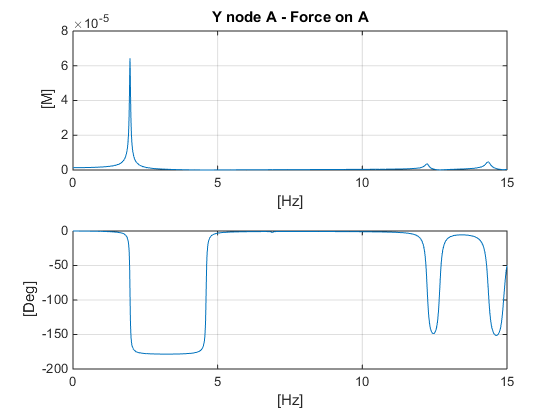
\includegraphics[width=\textwidth]{bode1}
                \caption{$y$ displacement of node A}
                \label{fig:bode1}
        \end{subfigure}%
        \begin{subfigure}[t]{0.5\textwidth}
                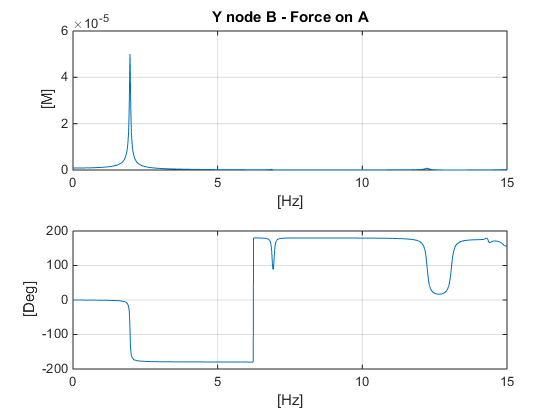
\includegraphics[width=\textwidth]{bode2}
                \caption{$y$ displacement of node B}
                \label{fig:bode2}
        \end{subfigure}
        \caption{FRF $y$ Displacement of nodes $A,B$ when a vertical force is applied on $A$, for $f \in [0,15]Hz$} \label{fig:bodes1}
\end{figure}\\
It's important to consider that we applied a force on node $A$. \\If we consider the displacement of node $A$ it's trivial to notice that the second frequency is not excited, due to the fact that $A$ is a nodal point for that natural frequency (figure \ref{fig:mode2}). For the last 3 frequencies node $ A$ is not a nodal point even though the modes of vibration associated to those frequencies have very small amplitude. \\If we consider the displacement of node $B$ for the second frequency we have that it's $0$ because node $A$ is a nodal point and we applied a force on $A$. For the third frequency node $B$ is not a nodal point even if it's near to being one. As for the other two frequencies we have that it's nearly a nodal point, therefore its FRF is $\approx 0$. \\ \\
Now we consider the acceleration of node $A,B$ when a force is applied on $B$:
\begin{figure}[h]
        \centering
        \begin{subfigure}[t]{0.5\textwidth}
                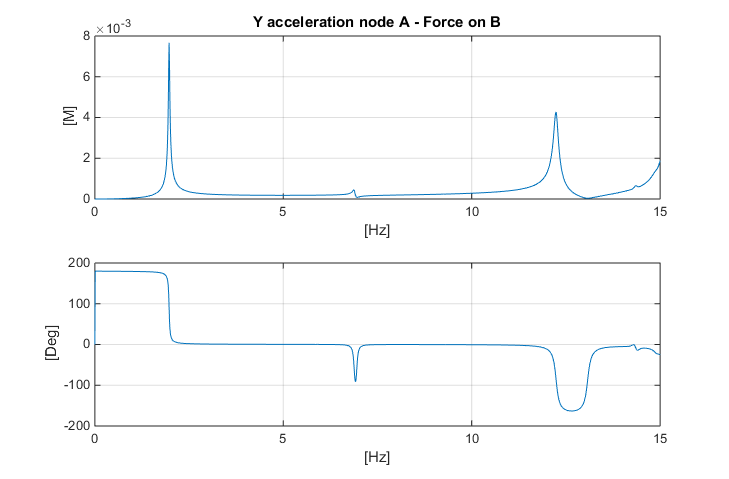
\includegraphics[width=\textwidth]{bode3}
                \caption{$y$ acceleration of node A}
                \label{fig:bode2}
        \end{subfigure}%
        \begin{subfigure}[t]{0.5\textwidth}
                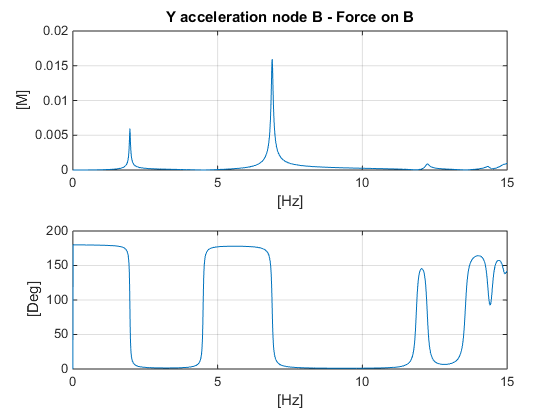
\includegraphics[width=\textwidth]{bode4}
                \caption{$y$ acceleration of node B}
                \label{fig:bode2}
        \end{subfigure}
        \caption{FRF $y$ acceleration of nodes $A,B$ when a vertical force is applied on $B$, for $f \in [0,15]Hz$} \label{fig:bodes2}
\end{figure}
\\
$A$ is a nodal point only for the second frequency whilst for all the others, and especially for the third one, we see peaks as expected. \\ 
$B$ is not a nodal point for the first two frequencies as we can see from the presence of two very high peaks. This happens because B is the point on which the force is applied. For the other two frequencies we have a near-nodal point situation and therefore its FRF is 0.

\newpage
\subsection{Earthquake analysis}
In this section we have to analyse the effect of a seismic motion of the ground applied on the bridge, specifically on the constrained nodes $O_1, O_2$. A picture of the $y$ displacement of those point is given in figure  \ref{fig:earthquake1}.

\begin{figure}[h]
\centering
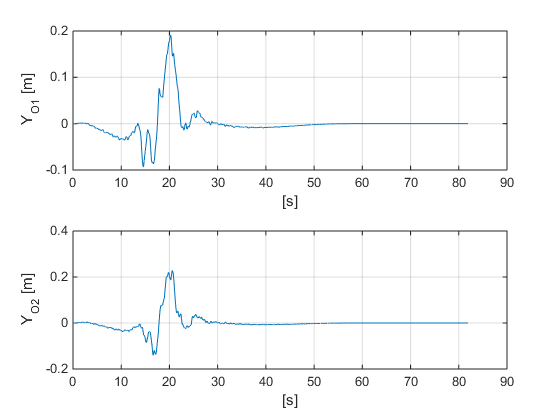
\includegraphics[scale=0.8]{earthquake1}
\label{fig:earthquake1}
\caption{Earthquake $y$ displacement of nodes $O_1,O_2$}
\end{figure}
If we consider the FFT (figure \ref{fig:earthquake2}, \ref{fig:earthquake3}) of these two signals, the frequency content of these signals is located in a neighbourhood of $0$, for this reason we'll consider frequencies $f \in [0,10] Hz$.

\begin{figure}[h]
        \centering
        \begin{subfigure}[t]{0.5\textwidth}
                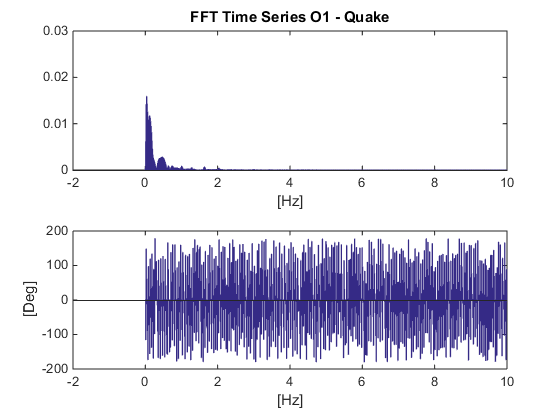
\includegraphics[width=\textwidth]{earthquake2}
                \caption{FFT earthquake in $O_1$}
                \label{fig:earthquake2}
        \end{subfigure}%
        \begin{subfigure}[t]{0.5\textwidth}
                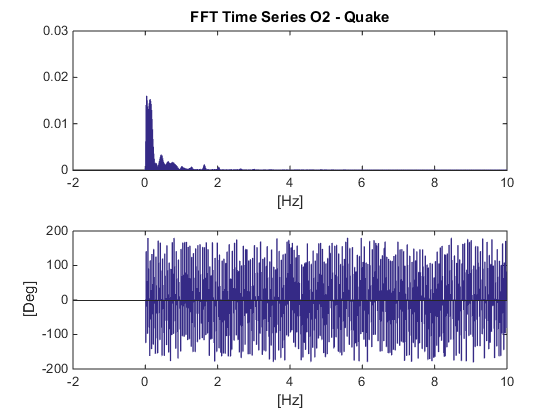
\includegraphics[width=\textwidth]{earthquake3}
                \caption{FFT earthquake in $O_2$}
                \label{fig:earthquake3}
        \end{subfigure}
         \label{fig:earthquake23}
\end{figure}
\newpage
The frequencies of the earthquake are well below the first natural frequency of the system, the displacements of nodes $A,B$ are:
\begin{figure}[h]
        \centering
        \begin{subfigure}[t]{0.5\textwidth}
                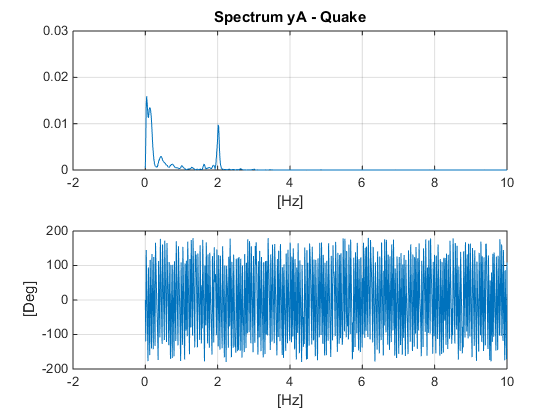
\includegraphics[width=\textwidth]{earthquake4}
                \caption{FFT earthquake in $A$}
                \label{fig:earthquake4}
        \end{subfigure}%
        \begin{subfigure}[t]{0.5\textwidth}
                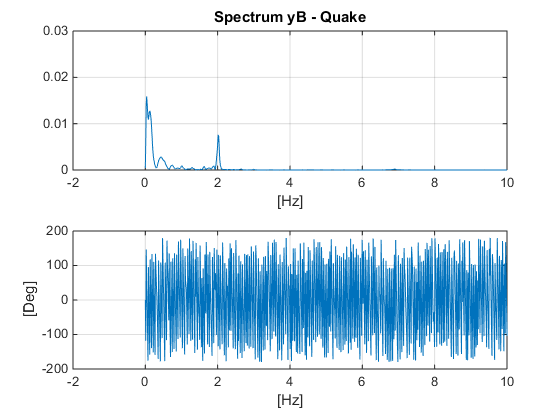
\includegraphics[width=\textwidth]{earthquake5}
                \caption{FFT earthquake in $B$}
                \label{fig:earthquake5}
        \end{subfigure}
         \label{fig:earthquake45}
\end{figure}

\begin{figure}[h]
        \centering
        \begin{subfigure}[t]{0.5\textwidth}
                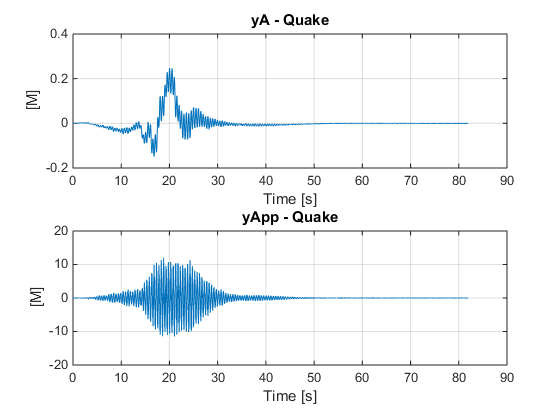
\includegraphics[width=\textwidth]{earthquake6}
                \caption{FFT earthquake in $A$}
                \label{fig:earthquake6}
        \end{subfigure}%
        \begin{subfigure}[t]{0.5\textwidth}
                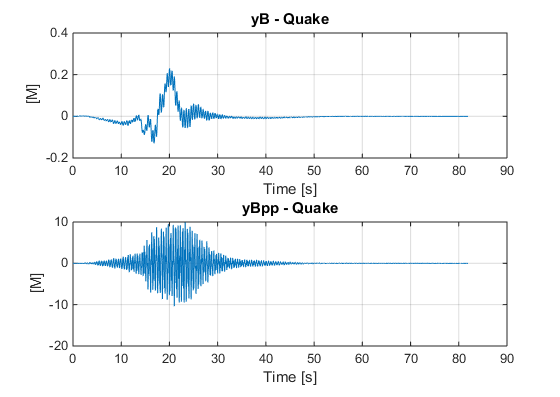
\includegraphics[width=\textwidth]{earthquake7}
                \caption{FFT earthquake in $B$}
                \label{fig:earthquake7}
        \end{subfigure}
         \label{fig:earthquake67}
\end{figure}
\newpage
\begin{lstlisting}
quake=load('sismaspost.txt');
plotQuake(quake);
t= (quake(:,1))';
yO1 = quake(:,2);
yO2 = quake(:,3);
N = size(quake,1);
T = quake(end,1);
fftO1 = fft(yO1);
fftO2 = fft(yO2);
df=1/T;
fmax = df*(N/2-1);
frequencies = (0:df:fmax)';

fftabsO1(1) = abs(fftO1(1))/N;
fftabsO2(1) = abs(fftO2(1))/N;
fftabsO1(2:N/2) = abs(fftO1(2:N/2))*2/N;
fftabsO2(2:N/2) = abs(fftO2(2:N/2))*2/N;
fftfasO1(1:N/2) = angle(fftO1(1:N/2));
fftfasO2(1:N/2) = angle(fftO2(1:N/2));
...    
for i =1:length(frequencies)
        omega = frequencies(i)*2*pi;
        XcO1 = fftabsO1(i)*exp(j*fftfasO1(i));
        XcO2 = fftabsO2(i)*exp(j*fftfasO2(i));
        Xc = [0; XcO1; XcO2];
        Qc = (-omega^2*Mfc+j*omega*Rfc+Kfc)*Xc;
        x = (-Mff*omega^2 +j*omega*Rff+Kff)\(-Qc);

        xa = x(NA);
        xb = x(NB);
        xapp = x(NA)*(-omega^2);
        xbpp = x(NB)*(-omega^2);

        moda(i) = abs(xa);
        modb(i) = abs(xb);
        modapp(i) = abs(xapp);
        modbpp(i) = abs(xbpp);


        fasa(i) = angle(xa);
        fasb(i) = angle(xb);
        fasapp(i) = angle(xapp);
        fasbpp(i) = angle(xbpp);

        qrO1 = qrO1+fftabsO1(i)*cos(omega*t+fftfasO1(i));
        yA = yA+ moda(i)*cos(omega*t+fasa(i));
        yApp = yApp+ modapp(i)*cos(omega*t+fasapp(i));
        yB = yB+ modb(i)*cos(omega*t+fasb(i));
        yBpp = yBpp+ modbpp(i)*cos(omega*t+fasbpp(i));
    end
\end{lstlisting}

\newpage
\subsection{Long Train passage}
The passage of a long train, with concentrated loads distancing $d=26m$ from one another can be mathematically modelled. For simplicity we assume the train to be infinitely long.\\ \\
The displacement of the $k$-eth load is given by the following formula:
$$x_{k}(t) = Vt-dk \quad k=0,1,\cdots$$
It's trivial to say that at any given time we have at most 3 loads on the bridge. As a matter of fact, when we have a load on $x=0$, since $d=26$, for $k=2$ we obtain $52$ while for $k=3$ $78$. \\
The only vertical force component acting on the bridge is due to gravity. \\ \\
\begin{tikzpicture}

% horizontal axis
\draw[->] (0,0) -- (7,0) node[anchor=north] {$t$};
% labels
\draw	(0,0) node[anchor=north] {0}
		(2,0) node[anchor=north] {$\frac{26}{V}$}
		(4,0) node[anchor=north] {$\frac{52}{V}$}
		(5.38,0) node[anchor=north] {$\frac{70}{V}$}
		(6,0) node[anchor=north] {$\frac{78}{V}$}
		(0,1) node[anchor=east] {$Mg$}
		(0,2) node[anchor=east] {$2Mg$}
		(0,3) node[anchor=east] {$3Mg$};
% ranges

% vertical axis
\draw[->] (0,0) -- (0,4) node[anchor=east] {$F_{y}$};
% nominal speed
\draw[dotted] (2,0) -- (2,1);
\draw[dotted] (4,0) -- (4,2);
\draw[dotted] (5.38,0) -- (5.38,2);
\draw[dotted] (6,0) -- (6,2);

% force
\draw[dotted] (0,1) -- (0,1);
\draw[dotted] (0,2) -- (2,2);
\draw[dotted] (0,3) -- (7,3);
% Us
\draw[thick] (0,0) -- (0,1) -- (2,1) -- (2,2) -- (4,2) -- (4,3) -- (5.38,3) -- (5.38,2) -- (6,2) -- (6,3) -- (7,3);

\end{tikzpicture}
\\
Notice that along the bridge the force is constant, whilst during the step we have an impulsive force acting either on $O_{1}$ or $O_{2}$.
Therefore, it is worth to study the effects on nodes $O_{1}$ and $O_{2}$. To this end we set up some analytical formulae that characterize this impulsive force. To do so we use the Dirac Impulse $\delta (t)$.
\\
Then, on $O_{1}$ , considering that the period is given by the formula $0=Vt-dk$,we have:
$$F_{y,O_{1}}(t) = \sum_{k=0}^{\infty} Mg\delta \big(t-kT\big),\quad T=\frac{d}{V} [s]$$
Similarly, for $O_{2}$, $70=Vt-dk$:
$$F_{y,O_{2}}(t) = \sum_{k=0}^{\infty} Mg\delta \big(t-kT-\hat{T}\big),\quad \hat{T}=\frac{70}{V}$$
In practice, $F_{y,O_{2}}(t) = F_{y,O_{1}}(t-\hat{T})$, as it should be. Thus we can study only $F_{y,O_{1}}(t)$ and we start by considering its spectrum. \\
\newpage
Consider the fourier series:
$$f(t) = \frac{a_0}{2} + \sum_{k=1}^{\infty} a_{k}cos(k\omega t)+b_{k}sin(k \omega t)$$
Where $f(t) =\sum_{k=0}^{\infty} Mg\delta \big(t-kT\big)$, $\omega = \frac{2\pi}{T}$.
The coefficients $a_{k},b_{k}$ are given by:
\begin{align*}
a_{k} &= \frac{2}{T} \int_{-\frac{T}{2}}^{\frac{T}{2}} f(t) cos(k\omega  t) dt \\
b_{k}&= \frac{2}{T} \int_{-\frac{T}{2}}^{\frac{T}{2}} f(t) sin(k\omega  t) dt
\end{align*}
Therefore $a_{k} = \frac{2Mg}{T}, b_{k}=0$:
\begin{align*}
f(t) = \frac{Mg}{T} + \sum_{k=1}^{\infty} \frac{2Mg}{T} cos(k\omega t)=\frac{Mg}{T}\sum_{k=-\infty}^{\infty} cos(k\omega t)=\frac{Mg}{T}\sum_{k=-\infty}^{\infty} e^{jk\omega t}
\end{align*}
Therefore the $FFT$ of the signal has $phase$ equal to $0$ and amplitude that is given by $\frac{Mg}{T}$, every $k\omega = k\frac{2\pi}{T}= k \frac{2\pi V}{d} = k\frac{\pi V}{13}$.
There might be resonance if $\exists k \in \mathbb{Z} : k\frac{\pi V}{13} \approx \omega_{i}$, where $\omega_{i}$ is a natural frequency of the system, $i=1,\cdots,n_{f}$. \\ \\
Consider now that $V \in [0,150] \frac{Km}{h} \Rightarrow V \in [0,41.67] \frac{m}{s}$, therefore:
$$k \stackrel{?}{\approx} \omega_{i} \frac{13}{\pi V}$$
To check if it is possible, consider the vector of natural frequencies of the system $\underline{\omega} = (\omega_{1}, \cdots \omega_{n})^T$ and the vector of the inverse of velocities $\underline{V}^{-1}= (\frac{1}{V_{1}}, \cdots,\frac{1}{V_{m}})^T$, where $n$ is the number of natural frequencies of the system, specifically the DOF, and $m$ the number of velocities considered.
We can construct a matrix $\mathbf{C} = \frac{13}{\pi}\underline{V}^{-1}\underline{\omega}^T$, where $C_{ij} = \frac{13\omega_{j}}{\pi V_{i}}$.
We can impose a rule with a parameter $\varepsilon > 0$ chosen by us, to define whenever there might be the chance of a resonance: $$min_{i,j} (|k\underline{1}\underline{1}^T - \mathbf{C} |)\leq \frac{13\varepsilon }{V\pi 2}=\overline{\varepsilon}$$
It's obvious to say that resonance happens, but for high values of $k$, for which there is an hyperbole that has the values of $V$ interesting to us for elevated $k$.\\ \\
Various tests were done on this code, especially to tests low frequency resonance. From these tests it results that the velocities that cause a resonance depend on the maximum velocity that can excit the $i$-eth natural frequency, which we will call $V_{max,i}$. The relationship is obviously hyperbolic, as previously stated. We can say from empirical tests that the $k$-eth 
velocity that excites the $i$-eth resonance frequency is of the form::
$$V_{res,k}=\frac{V_{max,i}}{1+ki^{-1}},\quad i = 1,2,3,\cdots\quad k=0,1,\cdots$$
From this a matrix can be built, where the $k,i$ cell represents the $k$-eth velocity  that excties the $i$-eth resonance frequency.
\begin{lstlisting}
v=1:0.01:55;
v=1./v;
freqk=freq(1);
Cn = 26*v'*freqk';
kmax = ceil(max(Cn(:)));
 sCn=size(Cn);
for k=1:kmax
   eps = abs(ones(sCn)*k - Cn);
   if (min(eps(:)) < 1e-5 *13*45/pi)
       [row,col] = find(eps == min(eps(:)));
       disp(['K: ' num2str(k) '- Matches: ' 
       num2str(length(find(eps<1e-5*13*45/pi))) '
        - [MIN]  Diff: ' num2str(eps(row,col)) ' 
        - Velocity: ' num2str(1/v(row)) ' 
        - Frequency: ' num2str(freq(col))]);
   end
end
\end{lstlisting}
\begin{figure}[h]
        \centering
        \begin{subfigure}[t]{0.5\textwidth}
                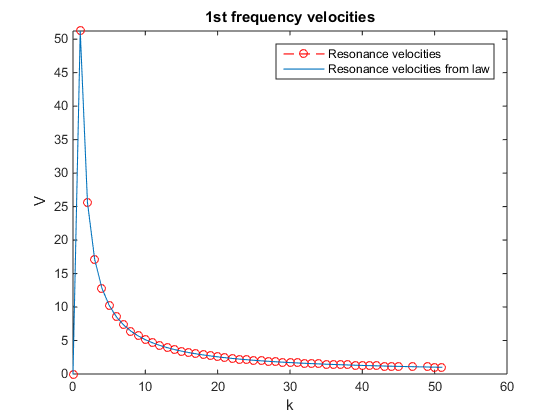
\includegraphics[width=\textwidth]{train1}
                \caption{1-st frequency resonance velocities}
                \label{fig:train1}
        \end{subfigure}%
        \begin{subfigure}[t]{0.5\textwidth}
                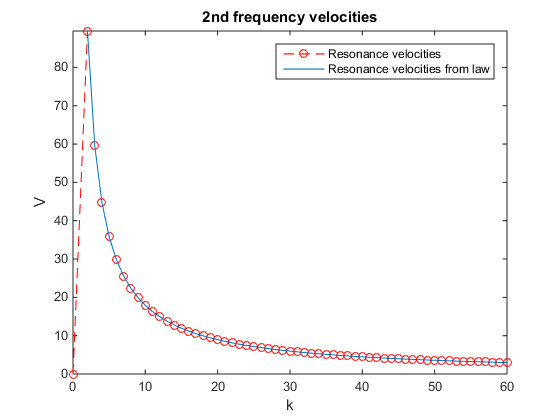
\includegraphics[width=\textwidth]{train2}
                \caption{2-nd frequency reosonance velocities}
                \label{fig:train2}
        \end{subfigure}
         \label{fig:train}
\end{figure}
A sample output given by the execution of the previous code is the following (for the first 4 frequencies, with velocity ranging from  $0$ to $100 \frac{m}{s}$):
\begin{lstlisting} [basicstyle=\fontsize{6}{5}\selectfont\ttfamily]
K: 1- Matches: 19 - [MIN]  Diff: 6.6453e-05 - Velocity: 51.22 - Frequency: 1.9701
K: 2- Matches: 21 - [MIN]  Diff: 7.7904e-05 - Velocity: 89.5 - Frequency: 6.8843
K: 3- Matches: 10 - [MIN]  Diff: 0.00021836 - Velocity: 59.66 - Frequency: 6.8843
K: 4- Matches: 22 - [MIN]  Diff: 7.8548e-06 - Velocity: 79.56 - Frequency: 12.24
K: 5- Matches: 13 - [MIN]  Diff: 0.00011786 - Velocity: 74.61 - Frequency: 14.3477
K: 6- Matches: 9 - [MIN]  Diff: 1.1782e-05 - Velocity: 53.04 - Frequency: 12.24
K: 7- Matches: 6 - [MIN]  Diff: 0.00011841 - Velocity: 25.57 - Frequency: 6.8843
...(output omitted)
\end{lstlisting}
\subsubsection{Modal approach verification}
It is possible to come up with the same solution using the modal approach. Remember that to using the modal approach means applying a linear trasformation to our coordinate $x, x=\Phi q$, where $q$ is the modal coordinate and $\Phi$ is the modal matrix containing the modes of vibration. \\
For beams the modal shape is $sin_k\Big(\frac{k\pi x}{L}\Big),k=1,\cdots$, where $L$ is the length of the beams' section considered and $k$ the $k$-eth modal shape. \\
In our case $x=Vt$ and the section of the beam we have to consider is $L=70m$. Moreover, since we have multiple trains, each one is $T=\frac{d}{V}$ seconds distant to the next train. Thus we obtain $sin_k\Big(\frac{k\pi(Vt-iT)}{L}\Big), i=0,\cdots$. \\ \\
Consider for simplicity just the first mode and the passage of 5 trains, then the generalized ecitation force is the following depicted in figure \ref{fig:train3} (which is the sum of the component of each train):
\begin{figure}[h]
        \centering
                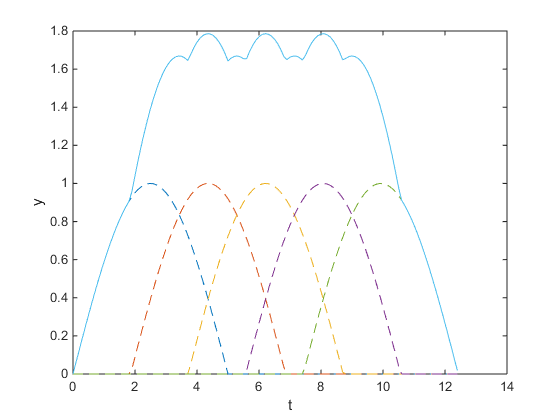
\includegraphics[width=\textwidth]{train3}
                \caption{Trend of the first generalized periodic excitation forces with 5 trains}
                \label{fig:train3}
\end{figure}
Since we considered only the first mode we obtain a concave parabola shape for each component. Moreover, each one lasts $Tmax=\frac{L}{V}$ and since we have $n$ trains then $Tmax =\frac{L}{V} + (n-1)\frac{d}{V}$.
\\ \\
It's straightforward to see that each sine has an offset of $T=\frac{d}{V}$ one another, therefore the excitation happens every $T$ seconds $\Rightarrow $ period $T$. If we take the the $FFT$ of such force the armonics are $\frac{k2\pi}{T} = \frac{2k\pi V}{d}$, which is like considering $d$ meters of the beam.\\
From this we obtain the same results previously reported.\newpage
For completeness, it is shown for the first frequency what happens for $V=\{51.22 ,25.6\} \frac{m}{s}$ which are resonance velocities and for $V=34 \frac{m}{s}$ which is not (notice that damping was not considered, and that images are not scaled, so check the amplitude):

\begin{figure}[h]
        \centering
        \begin{subfigure}[t]{0.5\textwidth}
                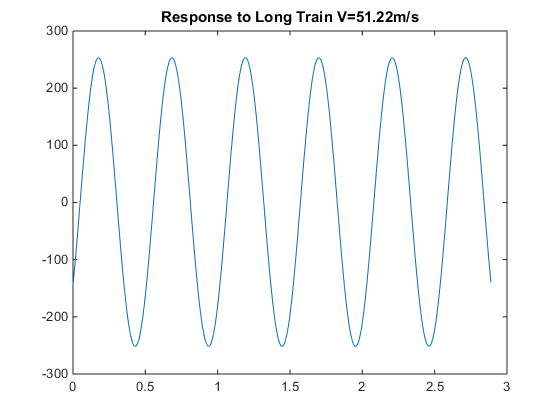
\includegraphics[width=\textwidth]{train4}
                \caption{Resonance velocity $V=51$m/s}
                \label{fig:earthquake4}
        \end{subfigure}%
        \begin{subfigure}[t]{0.5\textwidth}
                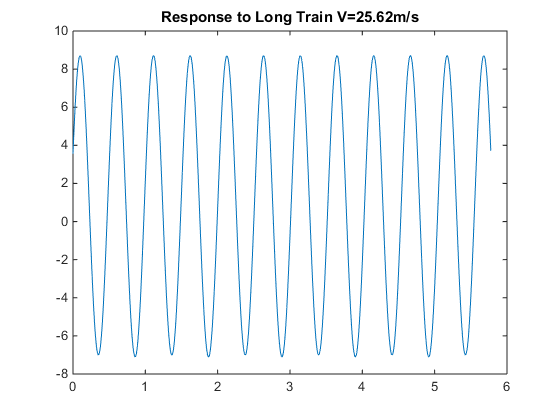
\includegraphics[width=\textwidth]{train5}
                \caption{Resonance velocity $V=25.6$m/s}
                \label{fig:earthquake5}
        \end{subfigure}
         \label{fig:earthquake45}
\end{figure}

\begin{figure}[h]
        \centering
        \begin{subfigure}[t]{0.5\textwidth}
                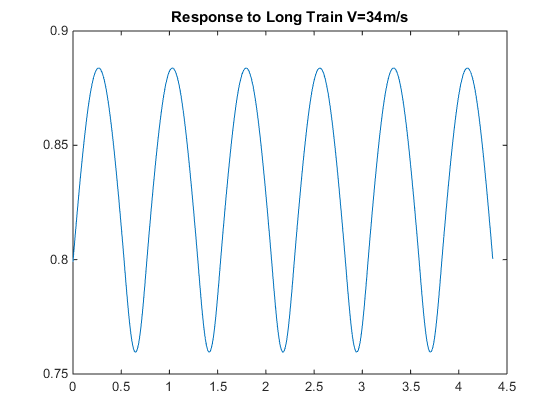
\includegraphics[width=\textwidth]{train6}
                \caption{Not resonant velocity $V=34$m/s}
                \label{fig:earthquake6}
        \end{subfigure}%
\end{figure}
\newpage
\subsection{Structural change}
In this part of the project we have to either make a structural change of the bridge in order to increase the first natural frequency by 20\% or to make a structural change on the bridge constraints to reduce by 15\% the maximum amplitude of vibration evaluated at point A when the bridge is subjected to the seismic excitation described at point 4.
\subsubsection{Structural change of the bridge}
The maximum increase in mass admitted is 3\%. Therefore, since the starting mass is $10990.4209 Kg$ the 3 \% increase is $11320 Kg$.
To do so it's important to observe that increasing the height of the bridge leads to an increase of the first natural frequency of the system. This is due to the fact that the beams are not parallel to the vertical axis, therefore they try to make the system oscillate along the vertical direction, then increasing the frequency of the vibration.
\\
Increasing the height by a factor of $1.3$ leads to a change of mass that is under the $3\%$, and the new mass is $11183.6377 Kg$. The new natural frequency is: $2.4987 Hz$. It's trivial to observe though that from a certain point onwards the horizontal oscillations prevail, leading to a reduction of the natural frequency (just imagine increasing the height to $\infty$)
\\
\begin{figure}[h]
        \centering
                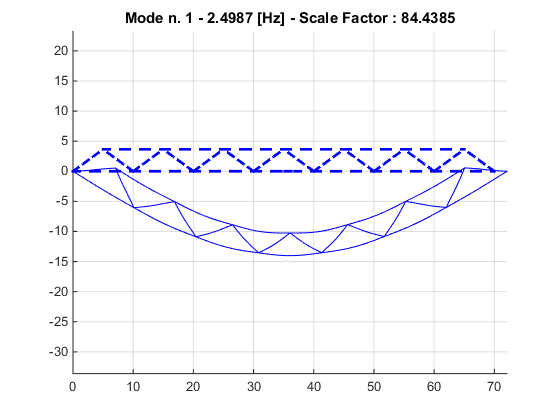
\includegraphics[width=\textwidth]{structuralchangea1}
                \caption{New natural frequency}
                \label{fig:newqfreqa}
\end{figure}
\subsubsection{Structural change of the constraints}
To increase the natural frequency by simply changing the constraint, it's trivial to observe that hindering the bridge to elongate on the horizontal direction leads to an automatic increase of the natural frequency (remember that the longer an object, the lower the natural frequencies $\Rightarrow$ if the bridge doesn't elongate, then we increase the frequencies). This can be done by replacing the cart on $O_2$ with a pin. 
\\
This leads to an increase of the first frequency up to $2.5 Hz$, and the reduction of the maximum amplitude of the quake is of about $35\%$. 
\\
In fact in point $4$ the maximum amplitude was $0.24727 m$, whilst now it's  $0.16095m$.\\
This is simple to understand since the quake has no frequency content in $2.5 Hz$. The same reasoning can be applied to point $6.a$.
\begin{figure}[h]
        \centering
        \begin{subfigure}[t]{0.5\textwidth}
                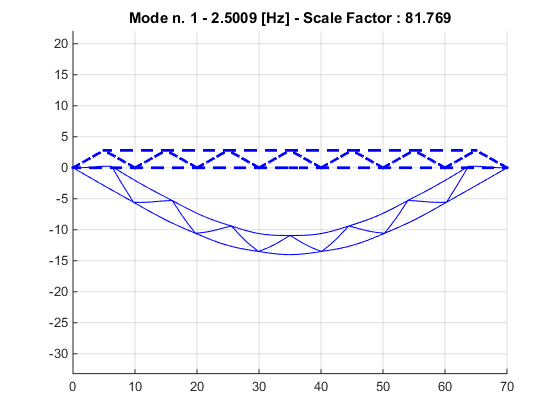
\includegraphics[width=\textwidth]{structuralchangeb1}
                \caption{New natural frequency}
                \label{fig:newqfreqb}
        \end{subfigure}%
        \begin{subfigure}[t]{0.5\textwidth}
                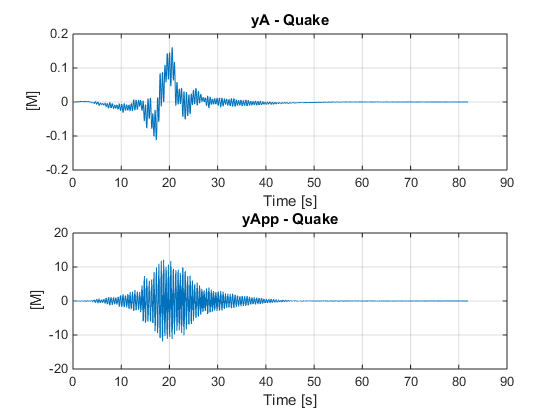
\includegraphics[width=\textwidth]{structuralchangeb2}
                \caption{$y$ displacement of Node A after the structural change}
                \label{fig:newquakeb}
        \end{subfigure}
         \label{fig:newa}
\end{figure}
\subsection{Previous version of the assignment}
The first request for the project was to reduce the maximum amplitude of vibration of node A when subjected to an earthquake of about 20\%, with a maximum increase of the bridge's mass of 5\%, which ends up being $11540$Kg. The difference is that it was modelled as a kart, with slider constraint and this meant that the first natural frequency was in the range of frequencies of the earthquake frequency content (see FRF of A in figure \ref{fig:last2}). This led to the maximum vibration of A being of $A$ being $0.2867cm$.\\
The first approach was to try changing the bridge's beams.\\
From the natural frequencies formula there is a direct evidence that reducing $J$ and increasing $m$ decreases the natural frequencies. Remember that $m=\rho A$, so we have a linear mass density.\\ \\
To do so the bottom and top beams were replaced with a beam type \textbf{IPE 220}, which has larger section and lower inertia.
\\
This leads to a bridge of mass $11657Kg$ but with a natural frequency of $1.9817Hz$.This, however, was not enough, since it reduced by $4cm$ the maximum amplitude (about 15\%).
\\ \\
To improve the bridge the diagonal beams were modified. Some beams were replaced with the \textbf{HEB 120}, which have lower area and inertia (the inertia in particular is much lower, about 1 order of magnitude, while the area changed by 10\%). This led to a bridge with acceptable mass, but instead of 
decreasing, the natural frequency rose. This is due to diagonal beams vibrating along the y axis. Higher frequencies are thus preferred. Some \textbf{HEB 140}  beams were then added, these have larger mass and about the same inertia as \textbf{HEB 120}.  The bridge mass then was $11519Kg$ and the first natural frequency was $1.968Hz$. Again, the maximum reduction of amplitude was of about $4.5-5cm$, which again is reasonable since it's the same first frequency of the hinge,kart constraint.
\begin{figure}[h]
        \centering
        \begin{subfigure}[t]{0.5\textwidth}
                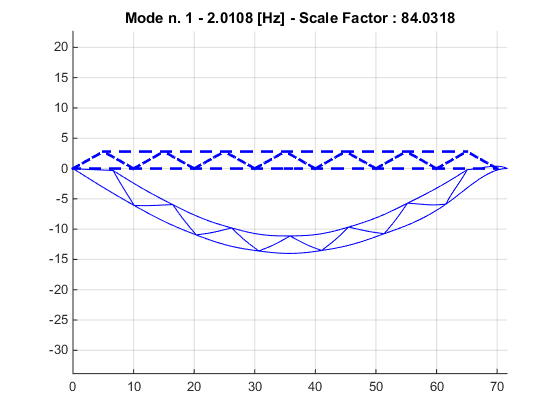
\includegraphics[width=\textwidth]{bridgelast0}
                \caption{First natural frequency with hinge,slider constraints}
                \label{fig:last1}
        \end{subfigure}%
        \begin{subfigure}[t]{0.5\textwidth}
                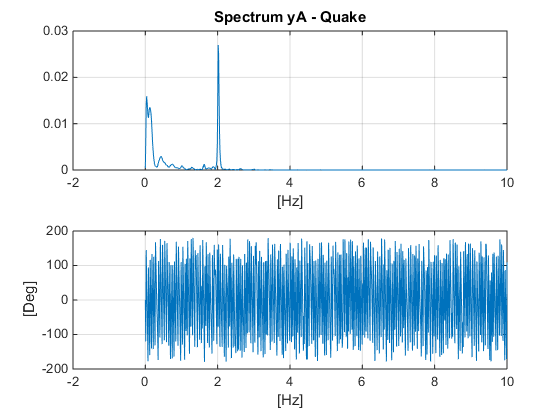
\includegraphics[width=\textwidth]{bridgelast01}
                \caption{FFT node A when subjected to an earthquake}
                \label{fig:last2}
        \end{subfigure}
         \label{fig:lasta}
\end{figure}
\begin{figure}[h]
        \centering
        \begin{subfigure}[t]{0.5\textwidth}
                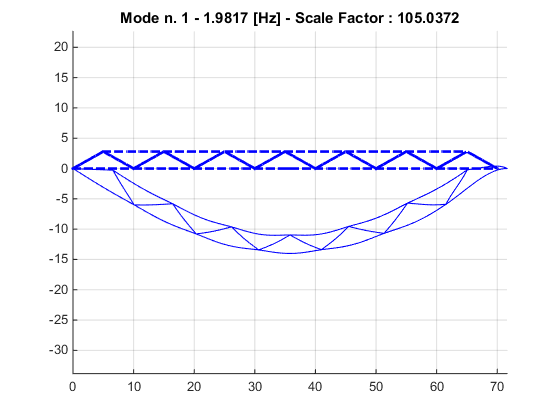
\includegraphics[width=\textwidth]{bridgelast1}
                \caption{First natural frequency after first change}
                \label{fig:last3}
        \end{subfigure}%
        \begin{subfigure}[t]{0.5\textwidth}
                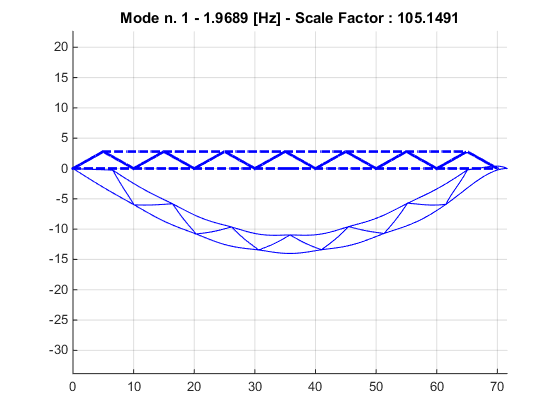
\includegraphics[width=\textwidth]{bridgelast2}
                \caption{First natural frequency after all the changes}
                \label{fig:last4}
        \end{subfigure}
         \label{fig:lastb}
\end{figure}
\newpage
\section{Appendix}
In the following sections I'll consider the analysis of the following function: $$g(s) = \frac{k\omega_0^2}{s^2+2 \xi \omega_0 s+\omega_0^2} \quad s \in \mathbb{C} , k \in \mathbb{R}, 0 \leq \xi \leq 1, \omega_0 = 2\pi f_0 \geq 0$$
By setting $s=j2\pi f$ we obtain:
$$ T(f)=g(j2\pi f)= \frac{k}{\big(1-\frac{f^2}{f_0^2}+j\frac{2\xi f}{f_0}\big)}$$
The modulus of $T$ is given by:
$$|T(f)|= \frac{|k|}{\sqrt{(1-\frac{f^2}{f_0^2})^2+(\frac{2\xi f}{f_0})^2}}$$.
\newpage
\subsection{Half-Power Rule}
This rule determines when the resonance peak's power drops by $\frac{1}{2}$. For this reason we consider a resonance peak with damping coefficient $\xi$ equal to $0$ and $k=1$.\\
Therefore the problem is to find the values of $f$ such that:
$$ |T(f)| = \frac{\sqrt{2}}{2} = \frac{1}{\sqrt{2}}$$
The following steps are trivial:
$$2|T(f)|^2=1 \Rightarrow 2 T(f)^2=1$$
We obtain:
\
$$ 2 = \Big(1-\frac{f^2}{f_0^2}\Big)^2 = 1+ \frac{f^4}{f_0^4}-2\frac{f^2}{f_0^2}$$
By setting $z=f^2$ and by multiplying for $f_0^4$:
$$z^2-2zf_0^2-f_0^4=0$$
Then:
$$ z_{1,2} = \frac{2f_0^2 \pm \sqrt{4f_0^4+4f_0^4}}{2} = f_0^2(1 \pm \sqrt{2})$$
$$
\Rightarrow f = \pm \sqrt{f_0^2(1 \pm \sqrt{2})}$$
\newpage
\subsection{Derivative Rule}
This method determines when the slope of the resonance peak is nearly the value given by the user, which we will call $m$.
For simplicity we'll assume $\xi = 0.$
\begin{gather*}
\frac{d}{df} |T(f)| = m \\
\frac{d}{df} \frac{|k|}{\sqrt{(1-\frac{f^2}{f_0^2})^2}} = m
\end{gather*}
Therefore:
\begin{align*}
\frac{d}{df} |T(f)| &= |k| \frac{-\frac{d}{df} {\sqrt{(1-\frac{f^2}{f_0^2})^2}}}{(1-\frac{f^2}{f_0^2})^2} =
|k| \frac{-\big(-\frac{2f}{f_0^2}\big)2\big(1-\frac{f^2}{f_0^2}\big)\frac{1}{2}\frac{1}{(1-\frac{f^2}{f_0^2})^2}}{(1-\frac{f^2}{f_0^2})^2}
\\
&= \frac{2|k|}{f_0^2} \frac{f(1-\frac{f^2}{f_0^2})}{((1-\frac{f^2}{f_0^2})^2)^{\frac{3}{2}}}=\frac{2|k|}{f_0^2} \frac{f(1-\frac{f^2}{f_0^2})}{|(1-\frac{f^2}{f_0^2})|^3}=m
\end{align*}
We can do the semplification as long as we remember that we need to consider the sign, but $T(f)=T(-f)$, therefore we can proceed and use this rule thereafter:
\begin{align*}
\frac{2|k|}{f_0^2} \frac{f}{(1-\frac{f^2}{f_0^2})^2}=m
\end{align*}
By letting $\frac{2|k|}{mf_0^2} = \hat{k}$:
\begin{align*}
 1+\frac{f^4}{f_0^4}-2\frac{f^2}{f_0^2} = \hat{k}f \\ f^4-2f_0^2f^2-\hat{k}f_0^4 f+f_0^4=0
\end{align*}
From this point onward an approximation method is used, but matlab provides function for finding roots of a polynomial.
\\
Since we seek for a solution around $f_0$, a Taylor expansion in $f_0$ might be suitable:
\begin{align*}
W(f) &= f^4-2f_0^2f^2-\hat{k}f_0^4 f+f_0^4 \\
W(f_0) &= -\hat{k}f_0^5 \\
W'(f_0) &= -\hat{k}f_0^4 \\
W''(f_0) &=8f_0^2 \\
W^{'''}(f_0) &=24f_0
\end{align*}
So:
$$
W(f) \approx -\hat{k}f_0^5 -\hat{k}f_0^4(f-f_0)+4f_0^2(f-f_0)^2+4f_0(f-f_0)^3
$$
\begin{align*}
0&=-\hat{k}f_0^5 -\hat{k}f_0^4(f-f_0)+4f_0^2(f-f_0)^2+4f_0(f-f_0)^3 \\
0&= -\hat{k}f_0^3f +4f_0(f^2+f_0^2-2f_0f)+4(f^3-f_0^3+3f_0^2f-3f_0f^2) \\
0&= f(-\hat{k}f_0^3 +4f^2+4f_0^2-8f_0f) = f(-\hat{k}f_0^3 +4(f-f_0)^2)
\end{align*}
Finally:
$$-\hat{k}f_0^3 +4(f-f_0)^2 = 0 \Rightarrow f = f_0\pm \frac{1}{2} \sqrt{\hat{k}f_0^3}$$
Since $T(-f)=T(f)$ also $-f$ is solution.
\newpage
\subsection{BeamLength function}

\begin{lstlisting}
function [L] = beamLength(...)
%
% Parameters is a vector with parameters P,A,J,E 
%-> parameters = [P,A,J,E];
% Frequency denotes the frequency range to be approximated
% Approximation is a scale factor that multiplied by the frequency
% gives the approximation, by default is 1 decade (10)
%
% The formula is 2*pi*f = (pi/L)^2   * sqrt(E*J/M);
% Therefore L = sqrt(pi/(2*f)  * sqrt(E*J/M));

% switch(nargin)
%     case 2
%         approximation =10 ;
%     case 3 ;
%     otherwise
%         error('beamLength:TooManyInputs', ...
%         'requires at least 2 inputs');
% end

frequency = abs(frequency);
parameters = abs(parameters);
switch(approximationType)
    case ApproxType.HalfPower
        fmax = frequency*sqrt((1+sqrt(2)));
    case ApproxType.FreqRange
        fmax = frequency*approximationParam;
    case ApproxType.DerivativeRule
        a=frequency;
        k=approximationParam;
        r = roots([-k,0,3*a^2*k,0,-3*a^2*k,-4*a^2,k*a^6]);
        r = round(r*10000)/10000.0;
        fmax = r(real(r)>a & imag(r)==0);        
    otherwise
        fmax = frequency*10;
end


 
M = parameters(1)*parameters(2);
sq1 = sqrt(parameters(4)*parameters(3)/M);
L = sqrt(pi*sq1/(2*fmax));


end
\end{lstlisting}
\newpage
\section{BuildStructure function}
\begin{lstlisting}
function [] = buildStructure(fileName, dampingCoefficients, 
frequency, approximationType, approximationParam)
% Usage: buildstructure('file.txt',[a,b], ApproxType.DerivativeRule,
% 0.5);
%
%
%
    if nargin < 3 || nargin > 5
        error('buildStructure:TooManyInputs', ...
            'requires at least 3 inputs');
    end
    
    if (size(dampingCoefficients) ~= 2)
        error('buildStructure:WrongDampingCoefficients', ...
            'You need to provide atleast 2 parameters 
            for the damping coefficients');
    end
    
    dampingCoefficients = abs(dampingCoefficients);
    frequency = abs(frequency);
    
    if ~exist('approximationType','var')
        approximationType = ApproxType.HalfPower;
    else
        if (approximationType == ApproxType.HalfPower)
            approximationParam=0;
        elseif (approximationType == ApproxType.FreqRange)
            if ~exist('approximationParam','var') ||
             ~isreal(approximationParam)
                disp('Not supplied an approximation param
                 for FreqRange or it is not a number.
                  A default one is provided (10)');
                approximationParam = 10;
            end
           % approximationParam = abs(approximationParam);
        elseif (approximationType == ApproxType.DerivativeRule)
           if ~exist('approximationParam','var') || 
           ~isreal(approximationParam)
                disp('Not supplied an approximation param 
                for DerivativeRule or it is not a number.
                 A default one is provided (10)');
                approximationParam = 0.5;
            end
            approximationParam = abs(approximationParam);
        else
            error('buildStructure:WrongApproximationType', ...
                'Wrong approximation type');
        end
    end

    
    disp(['Damping Coefficients: ' num2str(dampingCoefficients(1)) 
    ' - ' num2str(dampingCoefficients(2))]);
    disp(['Approximation Type: ' char(approximationType)]);
    disp(['Approximation Parameter: ' num2str(approximationParam)]);

    beams = java.util.LinkedList;
    nodes = java.util.LinkedList;
   
    readStructure(fileName,beams.listIterator,nodes.listIterator);
    
    beams = unique(listToMatrix(beams),'rows');
    nodes = unique(listToMatrix(nodes),'rows');
    
    disp(['Read ' num2str(size(beams,1)) ' beams']);
    disp(['Read ' num2str(size(nodes,1)) ' nodes']);
    
    
    [nodesTree,beamsTree] = buildNodesStructure(beams,nodes,
    frequency,approximationType, approximationParam);
    writeStructure(fileName, nodesTree,beamsTree, 
    dampingCoefficients);
end


function [nodesTree,beamsTree] = buildNodesStructure(beams,nodes,
frequency,approximationType, approximationParam)
    
    [nodesTree,beamsTree] = (placeNodes(beams,nodes,frequency, 	   
    approximationType,approximationParam));  
    nodesTree=round(nodesTree*100)/100.0;
    nodesTreeSize = size(nodesTree,1);
    
    for i=1:nodesTreeSize
       for j=i+1:nodesTreeSize
          if (nodesTree(i,2:3)==nodesTree(j,2:3))
              temp= nodesTree(j,1);
              nodesTree(j,1) = nodesTree(i,1);
              
              for w=1:size(beamsTree,1)
                for z=1:2
                    if (beamsTree(w,z+1)==temp)
                        beamsTree(w,z+1)=nodesTree(i,1);
                    end
                end
              end
              
          end
       end
    end
    
    nodesTree = unique(nodesTree,'rows');
    
    nodesTreeSize = size(nodesTree,1);
    for i=1:nodesTreeSize-1
       if (nodesTree(i+1,1) > nodesTree(i,1)+1)
          temp = nodesTree(i+1,1);
          n = nodesTree(i,1)+1;
          nodesTree(i+1,1) = n;
          for j=1:size(beamsTree,1)
              for z=1:2
                  if (beamsTree(j,z+1)== temp)
                      beamsTree(j,z+1) = n;
                  end
              end
          end
          
       end
    end

end

function [nodesTree,beamsTree] = placeNodes(beams,nodes,frequency,
approximationType,approximationParam)
    j=1;
    k=1;
    w=1;
    q=0;
    beamsTree = zeros(1,6);
    for z=1:size(beams,1)
        beam = beams(z,:);
        nlength = beamLength(beam(5:end), frequency, 
        approximationType,approximationParam);
        nnodes = ceil(beam(4)/nlength);
        nlength = beam(4)/nnodes;
        nnodes=nnodes+1;
        bn = zeros(nnodes, 6);
        beam(3) = beam(3)*pi/180;
        q=0;
        for i=1:nnodes
          %  beam(1:3)
            bn(i,1) = w;
            bn(i,2) = beam(1)+nlength*(i-1)*cos(beam(3));
            bn(i,3) = beam(2)+nlength*(i-1)*sin(beam(3));
            bn(i,4:end) = [0,0,0];
            %bn
            
            
            beamsTree=placeNodesBeams(beamsTree,beam,j,i+q,nnodes
            ,w,k);
            %beamsTree(:,1:3)
            
            for p=1:size(nodes,1)
                if(nodes(p,1:2)==bn(i,2:3))
                    bn(i,4:end) = nodes(p,3:end);
                elseif ( i < nnodes)
                    angle = atan2((nodes(p,2)-beam(2)),(nodes(p,1)
                    			-beam(1)));
                    r1 = beam(3)-angle;
                    if (r1 < 1e-10)
                        x = nodes(p,1);
                        y = nodes(p,2);
                        x0 = bn(i,2)+nlength*cos(beam(3));
                        y0 = bn(i,3)+nlength*sin(beam(3));
                        if ( ((x < x0 && y <= y0 )
                         || (x <= x0 && y < y0 ) )
                        && ( (bn(i,2) < x && bn(i,3) <=y) 
                        ||  (bn(i,2) <= x && bn(i,3) <y)))
                            w=w+1;
                            q=q+1;
                            nnodes=nnodes+1;
                            bn = [bn; w, nodes(p,:)];
                            beamsTree=placeNodesBeams(beamsTree,beam
                            ,j,i+q,nnodes,w,k);
                        end
                    end
                end
            end
            
            w=w+1;
        end
        if j==1
            nodesTree = [ bn];
        else
            nodesTree = [nodesTree;bn];
        end
        j = j+nnodes-1;
        k=k+1;
    end
end

function [beamsTree] = placeNodesBeams(beamsTree,beam,j,i,nnodes,w,k)

    if i==1
        kn=nnodes-1;
        beamsTree= [beamsTree; k*ones(kn,1) zeros(kn,2)
         beam(5)*beam(6)*ones(kn,1) beam(8)*beam(6)*ones(kn,1)
          beam(8)*beam(7)*ones(kn,1)];
        if (j==1)
            beamsTree = beamsTree(2:end,:);
        end
        beamsTree(j+i-1, 2) =w;
        %5 = p, 6=A, 7=J, 8=E
    elseif i==nnodes
        beamsTree(j+i-2, 3) = w; 
    else
        if (size(beamsTree,1) == j+i-2)
            kn=1;
            beamsTree= [beamsTree; k*ones(kn,1) zeros(kn,2) 
            beam(5)*beam(6)*ones(kn,1) beam(8)*beam(6)*ones(kn,1) 
            beam(8)*beam(7)*ones(kn,1)];
        end
            beamsTree(j+i-1, 2) =  w;
            beamsTree(j+i-2, 3) =  w;
    end
end



function [A] = listToMatrix(list)
    if(list.size()>0)
        A=zeros(list.size(), size(list.get(0),1));
        for i=1:list.size()
           A(i,:) = str2num(list.get(i-1))'; 
        end
    end
end
%--------------

function [] = readStructure(fileName, beams, nodes)
    fID = fopen(fileName);
    
    if fID ~= 1
         tline = fgetl(fID);
         while ischar(tline)
            strs = strsplit(tline,{'(',',',')'},
            'CollapseDelimiters',true);
            strs = strrep(strs, ' ', '');
            strs = strs(~cellfun('isempty',strs));
            parseLine(strs,beams,nodes);
            tline = fgetl(fID);
         end
    else
       error(['Cannot open the file: ' fileName]); 
    end
    
    fclose(fID);
end

function [] = parseLine(line, beams,nodes)
    if size(line,2) > 0
        c = line(1,1);
        switch(c{:})
            case 'b'
                beams.add(line(2:end));
            case 'n'
                nodes.add(line(2:end));
            otherwise
                error(['Unidentified command found during the 
                parsing of the structure file']);
        end
    end
end

function [] = writeStructure(fileName,nodesTree, 
beamsTree, dampingCoefficients)
    fileName = strcat(fileName, '.inp');
    fID = fopen(fileName,'w');
    if fID ~= 1
        fprintf(fID, '*NODES\n');
        for i=1:size(nodesTree,1)
            fprintf(fID, '%d \t  %d %d %d \t %f \t %f\n', 
            nodesTree(i,1), nodesTree(i,4),nodesTree(i,5),
            nodesTree(i,6), nodesTree(i,2),nodesTree(i,3));
        end
        fprintf(fID, '*ENDNODES\n');
        fprintf(fID, '*BEAMS\n');
        for i=1:size(beamsTree,1)
            fprintf(fID, '%d \t \t %d %d \t %f \t %f \t %f\n', i,
             beamsTree(i,2), beamsTree(i,3),beamsTree(i,4),
             beamsTree(i,5), beamsTree(i,6));
        end
        fprintf(fID, '*ENDBEAMS\n');
        fprintf(fID, '*DAMPING\n');
        fprintf(fID, '%f %f\n', dampingCoefficients(1),
         dampingCoefficients(2));
    else
       error(['Cannot open the file: ' fileName]);
    end
    fclose(fID);
end


\end{lstlisting}
\newpage
\section{Project Function}
\begin{lstlisting}
clc; clear all;
%load('bridgeStructure.txt_mkr.mat');
%load('bridgeStructure.New_mkr.mat');
%load('bridgeStructure.Newb_mkr.mat');
%load('bridgeStructure.springs_mkr.mat');
%load('bridgeNew.txt_mkr.mat');
load('bridgetestlast.txt_mkr.mat');
close all;
% Node O1: 1
% Node A: 32
% Node B: 13
% Node O2: 64
alpha=0.2;
beta=1e-4;
A = 50; %32
B = 20;%13;
O1 = 1;
O2 =101;%64;

NA = idb(A,2);
NB = idb(B,2);
N01 = idb(O1,2);
N02 = idb(O2,2);

n = size(idb,1)*3;
nc = 4;
nf = n-nc;

Mff = M(1:nf,1:nf);
Kff = K(1:nf,1:nf);
Rff = R(1:nf,1:nf);

Mfc = M(1:nf, nf+1:nf+nc);
Kfc = K(1:nf, nf+1:nf+nc);
Rfc = R(1:nf, nf+1:nf+nc);

Mcf = M(nf+1:nf+nc, 1:nf);
Kcf = K(nf+1:nf+nc, 1:nf);
Rcf = R(nf+1:nf+nc, 1:nf);
Mcc = M(nf+1:nf+nc, nf+1:nf+nc);
Kcc = K(nf+1:nf+nc, nf+1:nf+nc);
Rcc = R(nf+1:nf+nc, nf+1:nf+nc);
%%
[v,d]=eig(Mff\Kff);
[omega,I]=sort(sqrt(diag(d)));
freq=omega/2/pi;
sysomega = omega;

% Anew = [zeros(nf,nf), eye(nf,nf); -Mff\Kff, -Mff\Rff];
%  [shapes2,puls2]=eig(Anew);
%  
%  [omega,I]=sort( diag(puls2) );
%  freq = unique(abs(imag(omega)/(2*pi)));
%%  
project3Question(nf,NA,NB,Mff,Rff,Kff);

project4Question(Mff,Mfc,Rff,Rfc,Kff,Kfc,NA,NB);

\end{lstlisting}
\newpage
\section{Project3 Function}
\begin{lstlisting}
function [] = project3Question(nf,NA,NB,Mff,Rff,Kff)

    df = 0.01;
    frequencies = (0:df:15)';
    %----------
    F= zeros(nf,1); F(NA,1) = 1; 
    for i=1:size(frequencies,1);
       omega = frequencies(i)*2*pi;
       x = (-omega^2*Mff+j*omega*Rff+Kff)\F;
       xa = x(NA);
       xb = x(NB);
       moda(i) = abs(xa);
       modb(i) = abs(xb);

       fasa(i) = angle(xa);
       fasb(i) = angle(xb);
    end

    figure;
    subplot 211; plot(frequencies, moda); grid; 
    xlabel('[Hz]'); ylabel('[M]'); title('Y node A - Force on A');
    subplot 212; plot (frequencies, fasa*180/pi); grid; 
    xlabel('[Hz]'); ylabel('[Deg]');

    figure;
    subplot 211; plot(frequencies, modb); grid;
     xlabel('[Hz]'); ylabel('[M]'); title('Y node B - Force on A');
    subplot 212; plot (frequencies, fasb*180/pi); grid;
     xlabel('[Hz]'); ylabel('[Deg]');

    %---------
    F= zeros(nf,1); F(NB,1) = 1; 
    for i=1:size(frequencies,1);
       omega = frequencies(i)*2*pi;
       x = (-omega^2*Mff+j*omega*Rff+Kff)\F;
       xa = x(NA)*(-omega^2);
       xb = x(NB)*(-omega^2);
       moda(i) = abs(xa);
       modb(i) = abs(xb);

       fasa(i) = angle(xa);
       fasb(i) = angle(xb);
    end

    figure;
    subplot 211; plot(frequencies, moda); grid; 
    xlabel('[Hz]'); ylabel('[M]');
     title('Y acceleration node A - Force on B');
    subplot 212; plot (frequencies, fasa*180/pi); grid; 
    xlabel('[Hz]'); ylabel('[Deg]');

    figure;
    subplot 211; plot(frequencies, modb); grid;
    xlabel('[Hz]'); ylabel('[M]'); 
    title('Y acceleration node B - Force on B');
    subplot 212; plot (frequencies, fasb*180/pi); grid; 
    xlabel('[Hz]'); ylabel('[Deg]');
end
\end{lstlisting}
\newpage
\section{Project 4}
\begin{lstlisting}
function [] = project4Question(Mff,Mfc,Rff,Rfc,Kff,Kfc,NA,NB)
    quake=load('sismaspost.txt');
    plotQuake(quake);
    t= (quake(:,1))';
    yO1 = quake(:,2);
    yO2 = quake(:,3);

    N = size(quake,1);
    T = quake(end,1);
    fftO1 = fft(yO1);
    fftO2 = fft(yO2);

    df=1/T;
    fmax = df*(N/2-1);

    frequencies = (0:df:fmax)';

    fftabsO1(1) = abs(fftO1(1))/N;
    fftabsO2(1) = abs(fftO2(1))/N;
    fftabsO1(2:N/2) = abs(fftO1(2:N/2))*2/N;
    fftabsO2(2:N/2) = abs(fftO2(2:N/2))*2/N;
    fftfasO1(1:N/2) = angle(fftO1(1:N/2));
    fftfasO2(1:N/2) = angle(fftO2(1:N/2));

    figure;
    subplot 211; bar(frequencies, fftabsO1); xlabel('[Hz]');
     title('FFT Time Series O1 - Quake');  axis([-2 10 0 0.03]);
    subplot 212; bar(frequencies, fftfasO1*180/pi); xlabel('[Hz]');
     ylabel('[Deg]');  axis([-2 10 -200 200]);


    figure;
    subplot 211; bar(frequencies, fftabsO2); xlabel('[Hz]');
     title('FFT Time Series O2 - Quake'); axis([-2 10 0 0.03]);
    subplot 212; bar(frequencies, fftfasO2*180/pi); xlabel('[Hz]');
     ylabel('[Deg]');  axis([-2 10 -200 200]);

    qrO1 = zeros(1,N);
    yA = zeros(1,N);
    yB = zeros(1,N);
    yApp = zeros(1,N);
    yBpp = zeros(1,N);
    for i =1:length(frequencies)
        omega = frequencies(i)*2*pi;
        XcO1 = fftabsO1(i)*exp(j*fftfasO1(i));
        XcO2 = fftabsO2(i)*exp(j*fftfasO2(i));
        Xc = [0; XcO1; XcO2;0];
        Qc = (-omega^2*Mfc+j*omega*Rfc+Kfc)*Xc;
        x = (-Mff*omega^2 +j*omega*Rff+Kff)\(-Qc);

        xa = x(NA);
        xb = x(NB);
        xapp = x(NA)*(-omega^2);
        xbpp = x(NB)*(-omega^2);

        moda(i) = abs(xa);
        modb(i) = abs(xb);
        modapp(i) = abs(xapp);
        modbpp(i) = abs(xbpp);


        fasa(i) = angle(xa);
        fasb(i) = angle(xb);
        fasapp(i) = angle(xapp);
        fasbpp(i) = angle(xbpp);

        qrO1 = qrO1+fftabsO1(i)*cos(omega*t+fftfasO1(i));
      %  if (frequencies(i) < 0.5)
            yA = yA+ moda(i)*cos(omega*t+fasa(i));
            yApp = yApp+ modapp(i)*cos(omega*t+fasapp(i));
            yB = yB+ modb(i)*cos(omega*t+fasb(i));
            yBpp = yBpp+ modbpp(i)*cos(omega*t+fasbpp(i));
       % end
    end
    
    figure;
    plot(t, qrO1); grid; xlabel('Time [s]'); ylabel('[M]'); 
    title('Quake in O1 rebuilt');

    figure;
    subplot 211; plot(frequencies, moda); grid; xlabel('[Hz]');
     title('Spectrum yA - Quake'); axis([-2 10 0 0.03]);
    subplot 212; plot(frequencies, fasa*180/pi); grid;
     xlabel('[Hz]'); 
    ylabel('[Deg]');  axis([-2 10 -200 200]);


    figure;
    subplot 211; plot(frequencies, modapp); grid; xlabel('[Hz]');
     title('Spectrum yApp - Quake'); axis([-2 10 0 2]);
    subplot 212; plot(frequencies, fasapp*180/pi); grid;
     xlabel('[Hz]');
     ylabel('[Deg]');   axis([-2 10 -200 200]);

    figure;


    subplot 211; plot(frequencies, modb); grid; xlabel('[Hz]'); 
    title('Spectrum yB - Quake'); axis([-2 10 0 0.03]);
    subplot 212; plot(frequencies, fasb*180/pi); grid;
     xlabel('[Hz]');
     ylabel('[Deg]');  axis([-2 10 -200 200]);

    figure;


    subplot 211; plot(frequencies, modbpp); grid; xlabel('[Hz]');
     title('Spectrum yBpp - Quake'); axis([-2 10 0 2]);
    subplot 212; plot(frequencies, fasbpp*180/pi); grid;
    xlabel('[Hz]'); 
    ylabel('[Deg]');  axis([-2 10 -200 200]);

    figure;
    subplot 211; plot(t, yA);grid;xlabel('Time [s]'); 
    ylabel('[M]'); title('yA - Quake');
    subplot 212; plot(t,yApp);grid;xlabel('Time [s]'); 
    ylabel('[M]'); title('yApp - Quake');

    figure;
    subplot 211; plot(t, yB);grid;xlabel('Time [s]');
     ylabel('[M]'); title('yB - Quake');
    subplot 212; plot(t,yBpp);grid;xlabel('Time [s]'); 
    ylabel('[M]'); title('yBpp - Quake');

    figure;
    subplot 211; plot(t,abs(yA-yB)); grid;xlabel('Time [s]');
     ylabel('[M]'); title('abs(yA-yB) - Quake');
    subplot 212; plot(t,abs(yApp-yBpp)); grid;xlabel('Time [s]'); 
    ylabel('[M]'); title('abs(yApp-yBpp) - Quake');
    disp(['Maximum yA: ' num2str(max(yA))]);
end
\end{lstlisting}
\newpage
\section{BridgeStructure tool file}
\begin{lstlisting}

(b,0,0,0,10,7800, 0.008446,0.00023130,2.06e11)
(b,10,0,0,10,7800, 0.008446,0.00023130,2.06e11)
(b,20,0,0,10,7800, 0.008446,0.00023130,2.06e11)
(b,30,0,0,10,7800, 0.008446,0.0002313030,2.06e11)
(b,40,0,0,10,7800, 0.008446,0.00023130,2.06e11)
(b,50,0,0,10,7800, 0.008446,0.00023130,2.06e11)
(b,60,0,0,10,7800, 0.008446,0.00023130,2.06e11)


(b,5,2.8,0,10,7800, 0.008446,0.00023130,2.06e11)
(b,15,2.8,0,10,7800, 0.008446,0.00023130,2.06e11)
(b,25,2.8,0,10,7800, 0.008446,0.00023130,2.06e11)
(b,35,2.8,0,10,7800, 0.008446,0.00023130,2.06e11)
(b,45,2.8,0,10,7800, 0.008446,0.00023130,2.06e11)
(b,55,2.8,0,10,7800, 0.008446,0.00023130,2.06e11)


(b,0,0,29.25,5.73,7800, 0.003877,0.00001673,2.06e11)
(b,10,0,150.75,5.73,7800, 0.003877,0.00001673,2.06e11)
(b,10,0,29.25,5.73,7800, 0.003877,0.00001673,2.06e11)
(b,20,0,150.75,5.73,7800, 0.003877,0.00001673,2.06e11)
(b,20,0,29.25,5.73,7800, 0.003877,0.00001673,2.06e11)
(b,30,0,150.75,5.73,7800, 0.003877,0.00001673,2.06e11)
(b,30,0,29.25,5.73,7800, 0.003877,0.00001673,2.06e11)
(b,40,0,150.75,5.73,7800, 0.003877,0.00001673,2.06e11)
(b,40,0,29.25,5.73,7800, 0.003877,0.00001673,2.06e11)
(b,50,0,150.75,5.73,7800, 0.003877,0.00001673,2.06e11)
(b,50,0,29.25,5.73,7800, 0.003877,0.00001673,2.06e11)
(b,60,0,150.75,5.73,7800, 0.003877,0.00001673,2.06e11)
(b,60,0,29.25,5.73,7800, 0.003877,0.00001673,2.06e11)
(b,70,0,150.75,5.73,7800, 0.003877,0.00001673,2.06e11)

(n,0,0,1,1,0) 
(n,70,0,0,1,1) 
(n,20,0,0,0,0)
(n,35,0,0,0,0)
\end{lstlisting}
\newpage
\section{FEM Model}
\begin{lstlisting}
*NODES
1 	  1 1 0 	 0.000000 	 0.000000
2 	  0 0 0 	 3.330000 	 0.000000
3 	  0 0 0 	 6.670000 	 0.000000
4 	  0 0 0 	 10.000000 	 0.000000
5 	  0 0 0 	 1.670000 	 0.930000
6 	  0 0 0 	 3.330000 	 1.870000
7 	  0 0 0 	 5.000000 	 2.800000
8 	  0 0 0 	 8.330000 	 2.800000
9 	  0 0 0 	 11.670000 	 2.800000
10 	  0 0 0 	 15.000000 	 2.800000
11 	  0 0 0 	 13.330000 	 0.000000
12 	  0 0 0 	 16.670000 	 0.000000
13 	  0 0 0 	 20.000000 	 0.000000
14 	  0 0 0 	 11.670000 	 0.930000
15 	  0 0 0 	 13.330000 	 1.870000
16 	  0 0 0 	 8.330000 	 0.930000
17 	  0 0 0 	 6.670000 	 1.870000
18 	  0 0 0 	 18.330000 	 2.800000
19 	  0 0 0 	 21.670000 	 2.800000
20 	  0 0 0 	 25.000000 	 2.800000
21 	  0 0 0 	 23.330000 	 0.000000
22 	  0 0 0 	 26.670000 	 0.000000
23 	  0 0 0 	 30.000000 	 0.000000
24 	  0 0 0 	 21.670000 	 0.930000
25 	  0 0 0 	 23.330000 	 1.870000
26 	  0 0 0 	 18.330000 	 0.930000
27 	  0 0 0 	 16.670000 	 1.870000
28 	  0 0 0 	 28.330000 	 2.800000
29 	  0 0 0 	 31.670000 	 2.800000
30 	  0 0 0 	 35.000000 	 2.800000
31 	  0 0 0 	 33.330000 	 0.000000
32 	  0 0 0 	 35.000000 	 0.000000
33 	  0 0 0 	 36.670000 	 0.000000
34 	  0 0 0 	 40.000000 	 0.000000
35 	  0 0 0 	 31.670000 	 0.930000
36 	  0 0 0 	 33.330000 	 1.870000
37 	  0 0 0 	 28.330000 	 0.930000
38 	  0 0 0 	 26.670000 	 1.870000
39 	  0 0 0 	 38.330000 	 2.800000
40 	  0 0 0 	 41.670000 	 2.800000
41 	  0 0 0 	 45.000000 	 2.800000
42 	  0 0 0 	 43.330000 	 0.000000
43 	  0 0 0 	 46.670000 	 0.000000
44 	  0 0 0 	 50.000000 	 0.000000
45 	  0 0 0 	 41.670000 	 0.930000
46 	  0 0 0 	 43.330000 	 1.870000
47 	  0 0 0 	 38.330000 	 0.930000
48 	  0 0 0 	 36.670000 	 1.870000
49 	  0 0 0 	 48.330000 	 2.800000
50 	  0 0 0 	 51.670000 	 2.800000
51 	  0 0 0 	 55.000000 	 2.800000
52 	  0 0 0 	 53.330000 	 0.000000
53 	  0 0 0 	 56.670000 	 0.000000
54 	  0 0 0 	 60.000000 	 0.000000
55 	  0 0 0 	 51.670000 	 0.930000
56 	  0 0 0 	 53.330000 	 1.870000
57 	  0 0 0 	 48.330000 	 0.930000
58 	  0 0 0 	 46.670000 	 1.870000
59 	  0 0 0 	 58.330000 	 2.800000
60 	  0 0 0 	 61.670000 	 2.800000
61 	  0 0 0 	 65.000000 	 2.800000
62 	  0 0 0 	 63.330000 	 0.000000
63 	  0 0 0 	 66.670000 	 0.000000
64 	  0 1 0 	 70.000000 	 0.000000
65 	  0 0 0 	 61.670000 	 0.930000
66 	  0 0 0 	 63.330000 	 1.870000
67 	  0 0 0 	 58.330000 	 0.930000
68 	  0 0 0 	 56.670000 	 1.870000
69 	  0 0 0 	 68.330000 	 0.930000
70 	  0 0 0 	 66.670000 	 1.870000
*ENDNODES
*BEAMS
1 	 	 1 2 	 65.878800 	 1739876000.000000 	 47647800.000000
2 	 	 2 3 	 65.878800 	 1739876000.000000 	 47647800.000000
3 	 	 3 4 	 65.878800 	 1739876000.000000 	 47647800.000000
4 	 	 1 5 	 30.240600 	 798662000.000000 	 3446380.000000
5 	 	 5 6 	 30.240600 	 798662000.000000 	 3446380.000000
6 	 	 6 7 	 30.240600 	 798662000.000000 	 3446380.000000
7 	 	 7 8 	 65.878800 	 1739876000.000000 	 47647800.000000
8 	 	 8 9 	 65.878800 	 1739876000.000000 	 47647800.000000
9 	 	 9 10 	 65.878800 	 1739876000.000000 	 47647800.000000
10 	 	 4 11 	 65.878800 	 1739876000.000000 	 47647800.000000
11 	 	 11 12 	 65.878800 	 1739876000.000000 	 47647800.000000
12 	 	 12 13 	 65.878800 	 1739876000.000000 	 47647800.000000
13 	 	 4 14 	 30.240600 	 798662000.000000 	 3446380.000000
14 	 	 14 15 	 30.240600 	 798662000.000000 	 3446380.000000
15 	 	 15 10 	 30.240600 	 798662000.000000 	 3446380.000000
16 	 	 4 16 	 30.240600 	 798662000.000000 	 3446380.000000
17 	 	 16 17 	 30.240600 	 798662000.000000 	 3446380.000000
18 	 	 17 7 	 30.240600 	 798662000.000000 	 3446380.000000
19 	 	 10 18 	 65.878800 	 1739876000.000000 	 47647800.000000
20 	 	 18 19 	 65.878800 	 1739876000.000000 	 47647800.000000
21 	 	 19 20 	 65.878800 	 1739876000.000000 	 47647800.000000
22 	 	 13 21 	 65.878800 	 1739876000.000000 	 47647800.000000
23 	 	 21 22 	 65.878800 	 1739876000.000000 	 47647800.000000
24 	 	 22 23 	 65.878800 	 1739876000.000000 	 47647800.000000
25 	 	 13 24 	 30.240600 	 798662000.000000 	 3446380.000000
26 	 	 24 25 	 30.240600 	 798662000.000000 	 3446380.000000
27 	 	 25 20 	 30.240600 	 798662000.000000 	 3446380.000000
28 	 	 13 26 	 30.240600 	 798662000.000000 	 3446380.000000
29 	 	 26 27 	 30.240600 	 798662000.000000 	 3446380.000000
30 	 	 27 10 	 30.240600 	 798662000.000000 	 3446380.000000
31 	 	 20 28 	 65.878800 	 1739876000.000000 	 47647800.000000
32 	 	 28 29 	 65.878800 	 1739876000.000000 	 47647800.000000
33 	 	 29 30 	 65.878800 	 1739876000.000000 	 47647800.000000
34 	 	 23 31 	 65.878800 	 1739876000.000000 	 47647800.000000
35 	 	 31 32 	 65.878800 	 1739876000.000000 	 47647800.000000
36 	 	 32 33 	 65.878800 	 1739876000.000000 	 47647800.000000
37 	 	 33 34 	 65.878800 	 1739876000.000000 	 47647800.000000
38 	 	 23 35 	 30.240600 	 798662000.000000 	 3446380.000000
39 	 	 35 36 	 30.240600 	 798662000.000000 	 3446380.000000
40 	 	 36 30 	 30.240600 	 798662000.000000 	 3446380.000000
41 	 	 23 37 	 30.240600 	 798662000.000000 	 3446380.000000
42 	 	 37 38 	 30.240600 	 798662000.000000 	 3446380.000000
43 	 	 38 20 	 30.240600 	 798662000.000000 	 3446380.000000
44 	 	 30 39 	 65.878800 	 1739876000.000000 	 47647800.000000
45 	 	 39 40 	 65.878800 	 1739876000.000000 	 47647800.000000
46 	 	 40 41 	 65.878800 	 1739876000.000000 	 47647800.000000
47 	 	 34 42 	 65.878800 	 1739876000.000000 	 47647800.000000
48 	 	 42 43 	 65.878800 	 1739876000.000000 	 47647800.000000
49 	 	 43 44 	 65.878800 	 1739876000.000000 	 47647800.000000
50 	 	 34 45 	 30.240600 	 798662000.000000 	 3446380.000000
51 	 	 45 46 	 30.240600 	 798662000.000000 	 3446380.000000
52 	 	 46 41 	 30.240600 	 798662000.000000 	 3446380.000000
53 	 	 34 47 	 30.240600 	 798662000.000000 	 3446380.000000
54 	 	 47 48 	 30.240600 	 798662000.000000 	 3446380.000000
55 	 	 48 30 	 30.240600 	 798662000.000000 	 3446380.000000
56 	 	 41 49 	 65.878800 	 1739876000.000000 	 47647800.000000
57 	 	 49 50 	 65.878800 	 1739876000.000000 	 47647800.000000
58 	 	 50 51 	 65.878800 	 1739876000.000000 	 47647800.000000
59 	 	 44 52 	 65.878800 	 1739876000.000000 	 47647800.000000
60 	 	 52 53 	 65.878800 	 1739876000.000000 	 47647800.000000
61 	 	 53 54 	 65.878800 	 1739876000.000000 	 47647800.000000
62 	 	 44 55 	 30.240600 	 798662000.000000 	 3446380.000000
63 	 	 55 56 	 30.240600 	 798662000.000000 	 3446380.000000
64 	 	 56 51 	 30.240600 	 798662000.000000 	 3446380.000000
65 	 	 44 57 	 30.240600 	 798662000.000000 	 3446380.000000
66 	 	 57 58 	 30.240600 	 798662000.000000 	 3446380.000000
67 	 	 58 41 	 30.240600 	 798662000.000000 	 3446380.000000
68 	 	 51 59 	 65.878800 	 1739876000.000000 	 47647800.000000
69 	 	 59 60 	 65.878800 	 1739876000.000000 	 47647800.000000
70 	 	 60 61 	 65.878800 	 1739876000.000000 	 47647800.000000
71 	 	 54 62 	 65.878800 	 1739876000.000000 	 47647800.000000
72 	 	 62 63 	 65.878800 	 1739876000.000000 	 47647800.000000
73 	 	 63 64 	 65.878800 	 1739876000.000000 	 47647800.000000
74 	 	 54 65 	 30.240600 	 798662000.000000 	 3446380.000000
75 	 	 65 66 	 30.240600 	 798662000.000000 	 3446380.000000
76 	 	 66 61 	 30.240600 	 798662000.000000 	 3446380.000000
77 	 	 54 67 	 30.240600 	 798662000.000000 	 3446380.000000
78 	 	 67 68 	 30.240600 	 798662000.000000 	 3446380.000000
79 	 	 68 51 	 30.240600 	 798662000.000000 	 3446380.000000
80 	 	 64 69 	 30.240600 	 798662000.000000 	 3446380.000000
81 	 	 69 70 	 30.240600 	 798662000.000000 	 3446380.000000
82 	 	 70 61 	 30.240600 	 798662000.000000 	 3446380.000000
*ENDBEAMS
*DAMPING
0.200000 0.000100
\end{lstlisting}
\end{document}
